% !TeX root = ../../main.tex
\subsection{菱形刮板刮削效果评价}
\label{guaban_scraper_eval}
在工程应用中刮板相对于套管是直线运动，在实验室中复现该过程对设备要求高。考虑到工具上的主要功能结构——刮板通过与套管（垢）之间的相对运动产生清洁作用，在装置设计时抓住“相对运动”这一主要矛盾即可对刮板的使役性能进行模拟。

本项目设计了基于转盘的刮板刮削能力评价装置，其结构和工作原理如图\ref{fig:scraper_test_rig_mechanism}所示。该装置中，刮板与机架固连，铺设于转盘表面的垢主动旋转以产生相对运动（刮板的主切削运动）。刮板与垢之间是线（面）接触，二者并非严格意义上的相对平动，需对两者的差异作量级估算。转盘表面可视作套管内壁沿周向展开的平面：转盘切向（旋转方向）对应套管轴向即刮板行程方向，径向对应套管内壁的周向位置。本装置转盘半径为0.5 m，刮刀两端距盘心分别为$r_1 = 27\,\text{cm}$与$r_2 = 40\,\text{cm}$，接触区平均半径$\bar r=33.5$ cm。垢随转盘定轴转动时，接触区内各点的相对运动方向均沿切向且与刮刀刃线垂直，与直线平动在方向上一致。垢面上任一材料点的刮削仅发生在它经过刮刀正下方的瞬时接触过程中，对应的滑动距离等于刮刀刀齿沿运动方向的接触宽度$w$（毫米至厘米量级），远小于$\bar r$；在该接触过程中，材料点的运动路径为弧长$w$的圆弧，其相对直线的最大垂向偏差约为$w^2/(8\bar r)$（不超过0.1 mm），故局部刮削过程与直线平动等价。单次拉动刮痕的总长度由扇形垢样包角（约90°）决定，在垢样带内约为0.5 m，仅决定刮痕长度，不改变局部去除机理。接触区内沿刮刀径向跨度各点线速度$v=\omega r$不同，内、外端线速度之比$r_2/r_1\approx1.48$，相对平均速度的最大偏差约为$\pm19\%$，即当平均线速度约为0.05 m/s时，内、外端线速度分别约为0.040 m/s与0.060 m/s。该速度范围处于低速准静态区，硬垢的脆性崩碎去除机理对线速度不敏感。因此，以旋转盘面代替直线平动，对本节刮削效果的相对评价是可行的。

\begin{figure}[htbp]
	\centering
	\subfloat[实验装置结构及原理]{%
	\includegraphics[width=.9\textwidth]{figure/chapter3/scraper-test-rig.png}
	\label{fig:scraper_test_rig_mechanism}
	}
	\vspace{1em}
	\subfloat[弹簧变形量测量原理]{%
	\includegraphics[width=.9\textwidth]{figure/chapter3/scapter-measurement-mechanism.png}
	\label{fig:scapter_measurement_mechanism}
	}
	\caption{刮板刮削性能测试}
	\label{fig:scraper_test_rig}
\end{figure}

试验用垢样为模拟硬垢，其矿物成分以重晶石（硫酸钡）为主，用于近似模拟现场以硫酸钡/钡锶垢为主的坚硬垢层。制作时，将重晶石粉与硫铝酸盐水泥按质量比3:4干混均匀，加水拌合至浆体呈黏糊状态，浇注于放置在转盘盘面上的扇形模具中成形，养护至规定龄期后得到与转盘盘面粘接的扇形垢样。垢样位于距转盘中心半径30\textasciitilde{}38 cm的环形带内（内半径30 cm、外半径38 cm、厚度10 cm），垢样带外缘直径为0.76 m，本装置转盘半径为0.5 m（直径1 m），可满足垢样布置要求；扇形垢样沿周向的包角约为90°。为防止刮削过程中垢样边缘起翘、开裂或整体滑移，每块扇形垢样的两侧边缘均以环氧树脂与转盘盘面粘接固定。环氧树脂固定带及垢样台阶边缘处的刮削状态不具有代表性，故各测量点均布置在扇形垢样中部、距两侧环氧固定带一定距离的区域内，以保证刮削前后测量位置一致。垢样厚度（10 cm）远大于刮削深度（毫米级），刮削过程中垢层可视为半无限厚基体，转盘金属基底对刮削结果的影响可以忽略。为表征垢样的力学属性，同期以相同配比、相同工艺浇注了试块，用于测定垢样的抗压强度与硬度。

刮板是靠弹簧支撑的，为了模拟刮板的这种“浮动”支撑效果，在装置上设置了限位块约束刮板五个运动自由度，保留一个沿盘面法线方向的移动自由度。实验中，限位块用大跨距的横梁与机架固连，在刮板与垢之间的背向力较大时，可能产生挠曲变形$\delta _f$，需在计算弹簧压缩量$\delta_s$时进行补偿。

% 作者待补/核对：①扇形垢样块数及单次刮削流程（包角约90°、转盘半径0.5 m已确认）；②养护条件与龄期；③垢样抗压强度、硬度实测值及正文引用处；④刮刀刀齿沿运动方向接触宽度w的量级（正文按“毫米至厘米、垂向偏差不超过0.1 mm”定性表述，若实测请补具体值）；⑤手拉线速度0.05 m/s的测量位置（正文按接触区平均半径33.5 cm处表述）；⑥各尺寸测量基准面是否统一取垢样顶面。
实验记录的数据含义如图\ref{fig:scapter_measurement_mechanism}所示。实验前，先让弹簧处于原长状态，测量距离$l_{11}$和$l_{21}$，这两个尺寸分别是顶板顶部测量基面和限位块顶部、转盘盘面之间的距离。然后，根据弹簧的参考压缩量，将弹簧预紧，测量$l_{11}$、$l_{21}$，记为$l_{12}$、$l_{22}$。转动转盘，使刮板完成一次刮削过程，停止设备后，再次测量尺寸$l_{21}$，记为$l_{23}$。从实验台上取一个参考位置，在划痕的两侧取两个监测点，测量监测点相对于参考位置之间的距离$l_{31}$、$l_{32}$，再测量刮削坑的底部与参考点之间的距离$l_4$。实验中的尺寸测量采用的是精度为0.02 mm的游标卡尺，且刮削前后的尺寸测量均在同一扇形垢样区、同一测量位置完成，以保证测量基准一致。



根据几何关系，单次刮削产生的坑深度$\delta_c$、坑的累积深度$\delta_c'$，弹簧压缩量估计值$\delta_s$为
\begin{equation}
\centering
	\begin{aligned}
		\delta_c' & =l_4-\frac{l_{31}+l_{32}}{2}\\
		\delta_f & = l_{23}-l_{21}  \\ 
		\delta_s & = l_{11}-l_{12} - \delta_f- \delta_c'
	\end{aligned}
\end{equation}

垢经刮削后的形貌如图\ref{fig:scale_profile}所示。刮板前刀面附近堆积有粉末状和崩碎状屑，刀齿的容屑槽中也有此类屑，由此证明，所设计的刮板能有效刮除硬垢。在刮削区域的边缘也有这样的屑。从切屑的性质可以推测出，所设计的垢为脆性垢，与文献所述的垢性质吻合。%补充是哪一篇文献
从图中还可以看出，产屑量与弹簧的压缩量成正相关。
\begin{figure}[htbp]
	\centering
	\subfloat[$\delta_s=3.095\textrm{mm}$]{%
	\includegraphics[height=4.0cm]{figure/chapter3/scale-1.jpg}
	\label{fig:scale_1}
	}
	%\hfill
	\subfloat[$\delta_s=4.875\textrm{mm}$]{%
	\includegraphics[height=4.0cm]{figure/chapter3/scale-4.jpg}
	\label{fig:scale_4}
	}
	\\[1.2em]
	\subfloat[$\delta_s=5.155\textrm{mm}$]{%
	\includegraphics[height=4.0cm]{figure/chapter3/scale-3.jpg}
	\label{fig:scale_3}
	}
	%\hfill
	\subfloat[$\delta_s=6.465\textrm{mm}$]{%
	\includegraphics[height=4.0cm]{figure/chapter3/scale-5.jpg}
	\label{fig:scale_5}
	}	
	\caption{垢层经刮削后的表面形貌（不同弹簧压缩量）}
	\label{fig:scale_profile}
\end{figure}


此外，刮板表面的有效刮削功能单元是表面齿，总体上看，刮板主要依靠具有负前角的前刀面进行刮削，其余位置的齿起到辅助作用。刮削中产生的粉末状垢屑极易导致刮板上刀齿前刀面堵塞，如图\ref{fig:scraper_profile}所示。在清理垢时还发现，后刀面在弹簧的巨大预紧力作用下与垢强烈摩擦，后刀面附着有一层质地坚硬的垢变质层，其强度和硬度比垢基材高，在一定程度上减缓了后刀面的磨损。刮板前刀面附近的切削齿堵塞较为严重，增加弹簧的预紧力会加剧这种堵塞效果，这说明此刮板应容易堵塞。横向螺纹齿最容易被堵塞，斜向的三角齿由于容屑槽空间大，切削性能可保持的时间会更长。在实际应用中，可以推测，螺纹齿在刮削的初期就被堵塞而失效。主切削齿在初始阶段承担主要的刮削任务；随着刮削行程的增长，其主切削刃磨钝，三角齿主要起着刮削的作用。在实际应用中，如能建立循环不断冲洗刮板，将有助于屑从容屑槽中排出，对提高刮板的使用效能有促进作用。

\begin{figure}[htbp]
	\centering
	\subfloat[$\delta_s=3.095\textrm{mm}$]{%
	\includegraphics[width=.32\textwidth]{figure/chapter3/scraper-1.jpg}
	\label{fig:scraper_1}
	}
	%\hfill
	\subfloat[$\delta_s=4.875\textrm{mm}$]{%
	\includegraphics[width=.32\textwidth]{figure/chapter3/scraper-4.jpg}
	\label{fig:scraper_4}
	}
	\vspace{0em}
	\subfloat[$\delta_s=5.155\textrm{mm}$]{%
	\includegraphics[width=.32\textwidth]{figure/chapter3/scraper-3.jpg}
	\label{fig:scraper_3}
	}
	%\hfill
	\subfloat[$\delta_s=6.465\textrm{mm}$]{%
	\includegraphics[width=.32\textwidth]{figure/chapter3/scraper-5.jpg}
	\label{fig:scaper_5}
	}	
	\caption{刮削后刮板刀齿表面形貌及切屑堵塞情况}
	\label{fig:scraper_profile}
\end{figure}



本试验基于图\ref{fig:scraper_test_rig}所示的转盘式台架，以重晶石粉与硫铝酸盐水泥配制的模拟硬垢为对象，考察了弹簧压缩量对刮板刮削效果的影响。结果表明：所设计的刮板能够有效刮除该类硬垢，但单次刮削厚度并不随弹簧预紧量的增大而增大，而是随弹簧压缩量的增大而减小，并在某一压缩量附近出现陡降，说明实际应用中弹簧预紧量存在临界值与有效工作区间。

从装置与方法看，转盘旋转可在低速条件下复现刮板相对垢面的刮削运动：接触区内相对运动方向与直线平动一致，线速度沿刮刀跨度虽有约±19\%的变化，但处于低速准静态范围，不改变硬垢脆性崩碎的去除机理；结合弹簧变形量与刮痕深度的逐点测量，可定量评价不同预紧工况下的刮削效果，为刮管工具的台架评价提供了可行方法。

从刮削形貌看，刮削后的垢面呈连续规则的沟槽，刀齿前刀面与容屑槽内见粉末状及崩碎状切屑（图\ref{fig:scale_profile}），表明垢层以脆性崩碎方式去除，刮板具备对重晶石/钡锶类硬垢的实际刮除能力；同时可见，产屑量随弹簧压缩量的增大而增多，而细屑对刀齿前刀面、容屑槽的充填堵塞及垢面压实变质层的发育也随压缩量的增大而加剧（图\ref{fig:scraper_profile}），说明单纯增大预紧量并不能成比例地提高有效刮削能力，这与图\ref{fig:scratch_depth_spring_comprassion}所示的响应规律一致。

从单次刮削厚度随弹簧压缩估计值的响应看（图\ref{fig:scratch_depth_spring_comprassion}），二者并非单调递增关系，而呈“缓降—陡降—稳定”的三段特征：弹簧压缩量约为3.9 mm和5.5 mm时，单次刮削厚度分别约为0.85 mm和0.71 mm，降幅不大；压缩量增至约7.1 mm时，厚度约为0.64 mm；压缩量进一步增至约7.3 mm时，厚度骤降至约0.11 mm；此后（约9.6 mm）厚度基本稳定在0.08 mm左右。由此可知，弹簧预紧量存在临界值（本试验条件下约为7.2 mm）：在临界值以内，刀齿能够保持相对稳定的压入深度，单次刮削厚度随压缩量的增大缓慢减小；当压缩量接近并超过临界值后，一方面刀齿与垢面的实际接触面积显著增大、垢层表面被压实变质并产生大量细屑，细屑迅速充填刀齿前刀面与容屑槽（图\ref{fig:scraper_profile}），参与有效切削的齿减少；另一方面刮板的浮动支撑逐渐接近其径向行程极限，刀齿难以继续压入垢层，刮削中切削所占比重下降、挤压与摩擦所占比重上升，单次刮削厚度急剧下降并趋于稳定。需要说明的是，本文各工况在同一扇形垢样、同一沟槽上依次进行，弹簧压缩量随工况逐步调整，图中反映的是弹簧压缩量对刮削厚度的总体影响趋势。

面向工程应用，弹簧预紧量不宜盲目加大，而应控制在其有效区间内：预紧量过小，刀齿难以始终贴紧壁面，清洁能力受限；预紧量过大，单次刮削厚度不升反降，并会因齿面堵塞和浮动支撑压死使刮削能力骤降，同时加剧刀齿与后刀面的磨损。按本节试验结果，弹簧压缩量在约$4\sim7$ mm范围内时，单次刮削厚度保持在较高水平且变化平缓，可作为该刮板预紧量的推荐工作区间；实际应用中还应结合套管的实际内径（同一公称尺寸不同线重时内径不同）匹配刮刀外径与弹簧预紧量，使弹簧压缩量不超过临界值，避免盲目增大预紧力；现场作业宜配合循环冲洗及时排屑，以延缓齿面堵塞、延长刮板有效使用寿命。

综上，研制的刮板对重晶石/钡锶类硬垢刮削有效，转盘台架及其测量方法可用于刮板刮削能力的相对评价；单次刮削厚度随弹簧压缩量的增大而减小，并在约7.2 mm附近出现陡降，说明弹簧预紧量存在临界值，实际应用中应结合套管规格匹配刮刀外径与弹簧预紧量、将弹簧压缩量控制在临界值以内，并辅以循环排屑措施。
\begin{figure}	
	\centering
	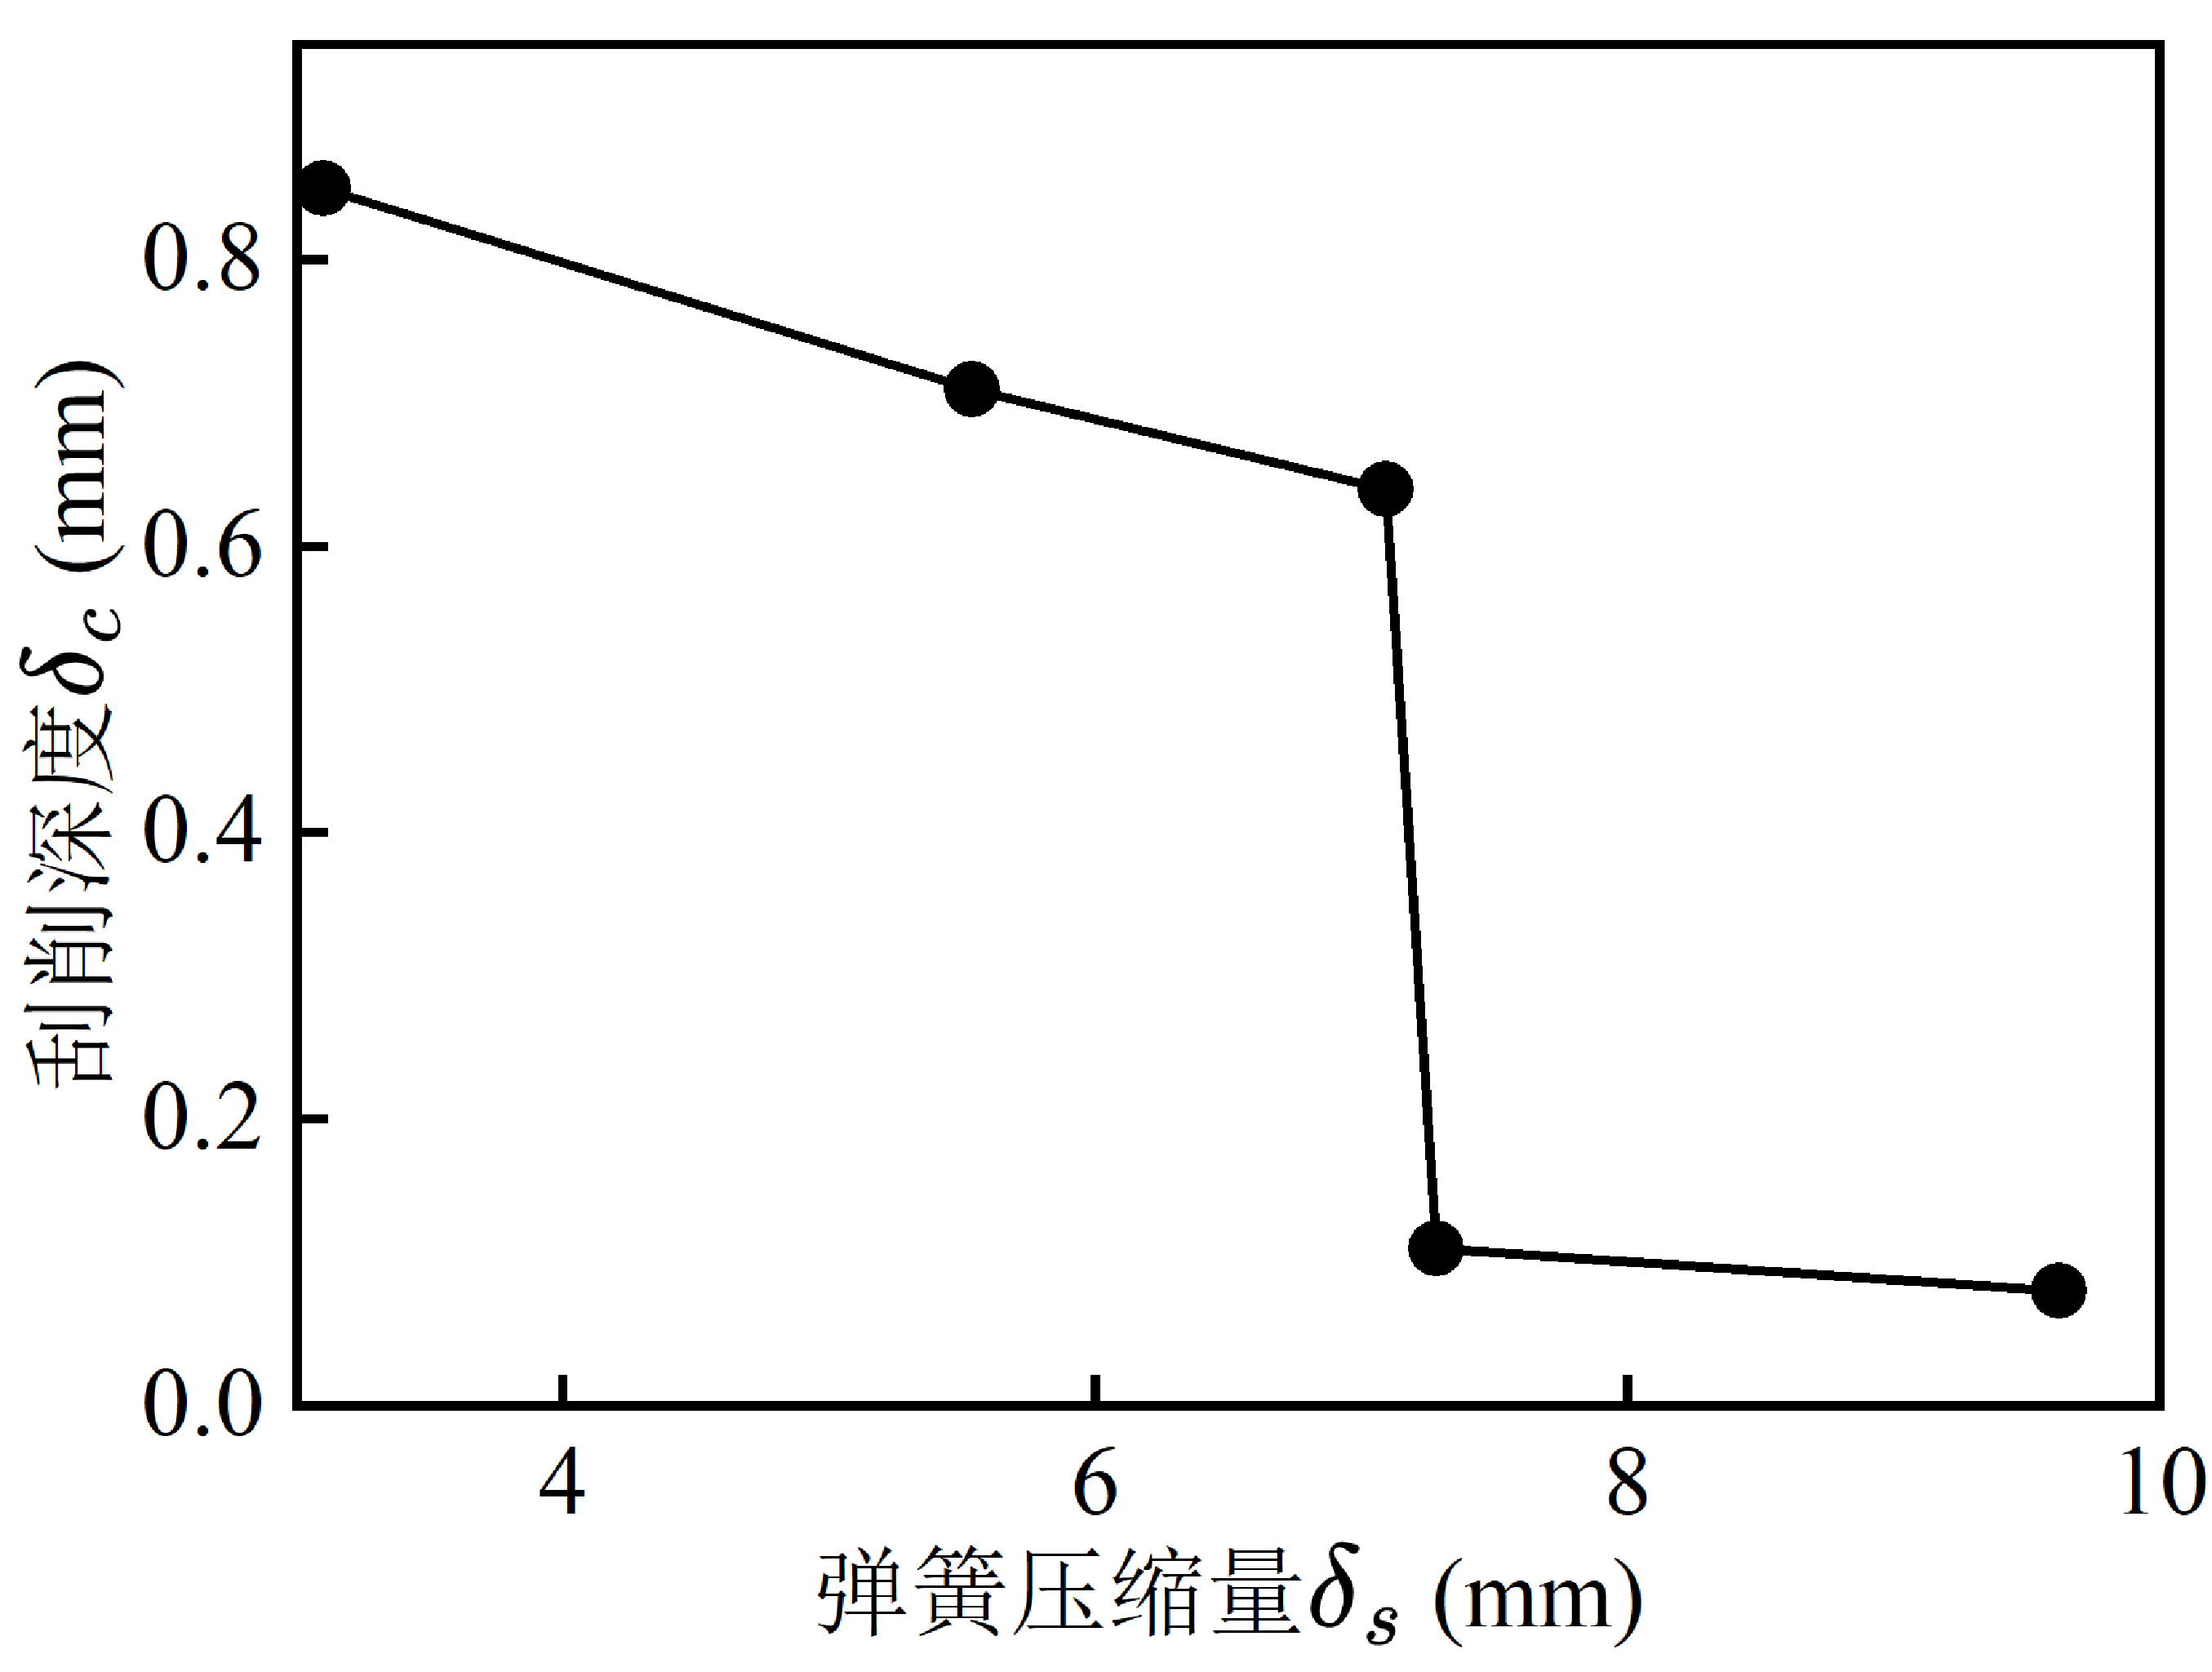
\includegraphics[width=.6\textwidth]{figure/chapter3/scatch-depth-sping-comprassion.png}
	\caption{刮削深度与弹簧压缩量之间的关系}
	\label{fig:scratch_depth_spring_comprassion}
\end{figure}

\subsection{斜齿形刮板刮削效果评价}
% 作者待补：斜齿形刮板评价装置结构及原理图（figure/chapter3/xiechiguaban/ 下暂无对应图片），暂以菱形刮板试验的转盘式台架图（fig:scraper_test_rig）代替，补充后其 \label 用 fig:helical_scraper_test_rig
与菱形刮板相比，斜齿形刮板的刀齿沿刮削方向呈螺旋状布置，刮削过程中刀齿与垢面接触的相对运动方向不再严格垂直于刮削方向，而是具有一定的切向分量。为评价斜齿形刮板的刮削效果，本项目在转盘式刮板刮削能力评价装置上开展斜齿形刮板的刮削试验，斜齿形刮板装夹于与菱形刮板试验相同的台架（图\ref{fig:scraper_test_rig}），台架的运动学与力学条件相同。该装置中，刮板与机架固连，铺设于转盘表面的垢主动旋转以产生相对运动（刮板的主切削运动）。
实验原理与菱形刮板相同，刮板与垢之间是线（面）接触，二者并非严格意义上的相对平动，需对两者的差异作量级估算。转盘表面可视作套管内壁沿周向展开的平面：转盘切向（旋转方向）对应套管轴向即刮板行程方向，径向对应套管内壁的周向位置。本装置转盘半径为0.5 m，刮刀两端距盘心分别为$r_1 = 27\,\text{cm}$与$r_2 = 40\,\text{cm}$，接触区平均半径$\bar r=33.5$ cm。垢随转盘定轴转动时，接触区内各点的相对运动方向均沿切向且与刮刀刃线垂直，与直线平动在方向上一致。

斜齿形刮板刮削后的垢面形貌如图\ref{fig:helical_scale_profile}所示。垢面上留有连续、排布整齐的刮痕，刮痕的延伸方向即为刮板相对垢面的运动方向；刮痕两侧的沟槽底部可见台阶状（梯形）残留形貌，这是斜齿形刮板中间并列布置的梯形齿在工作面上留下的轮廓。图中浅色、白色部分为尚未被刮除的垢样（垢面），其间深色的条带则是刀齿刮出的沟槽与工具金属表面，二者共同构成本节的刮削形貌。刀齿前刀面及容屑槽内附着有粉末状与崩碎状切屑，切屑的性状与菱形刮板试验中观察到的脆性崩碎屑一致，说明斜齿形刮板同样以脆性崩碎的方式去除垢层，对重晶石/钡锶类硬垢具有有效的刮除能力。从切屑在齿间的分布看，崩碎屑与细粉状附着物相对集中于两侧齿根部所在的平台处，中部容屑槽的排屑状况相对较好；结合斜齿形刮板刀齿呈螺旋状布置、齿间容屑与过流空间较大这一结构特点，可以认为其排屑条件优于齿槽相对封闭的横向螺纹齿，因而在高预紧工况下齿面被细屑完全充填、失去切削能力的风险更低。此外，对比不同弹簧压缩量下的形貌可见，随$\delta_s$由7.21 mm增大至10.11 mm、11.26 mm，垢面崩碎屑的量以及齿面附着的细粉状垢屑均相应增多，说明预紧量增大使齿间的产屑量与细屑附着量增多、齿面堵塞的风险上升，这与菱形刮板试验中产屑量随压缩量增大而增多的规律一致；但由后文的分析可知，斜齿形刮板的单次刮削厚度并不随预紧量的增大单调增大，产屑量的多少并不能直接反映单位行程的有效去除量。
\begin{figure}[htbp]
	\centering
	\subfloat[$\delta_s=7.21\textrm{mm}$]{%
	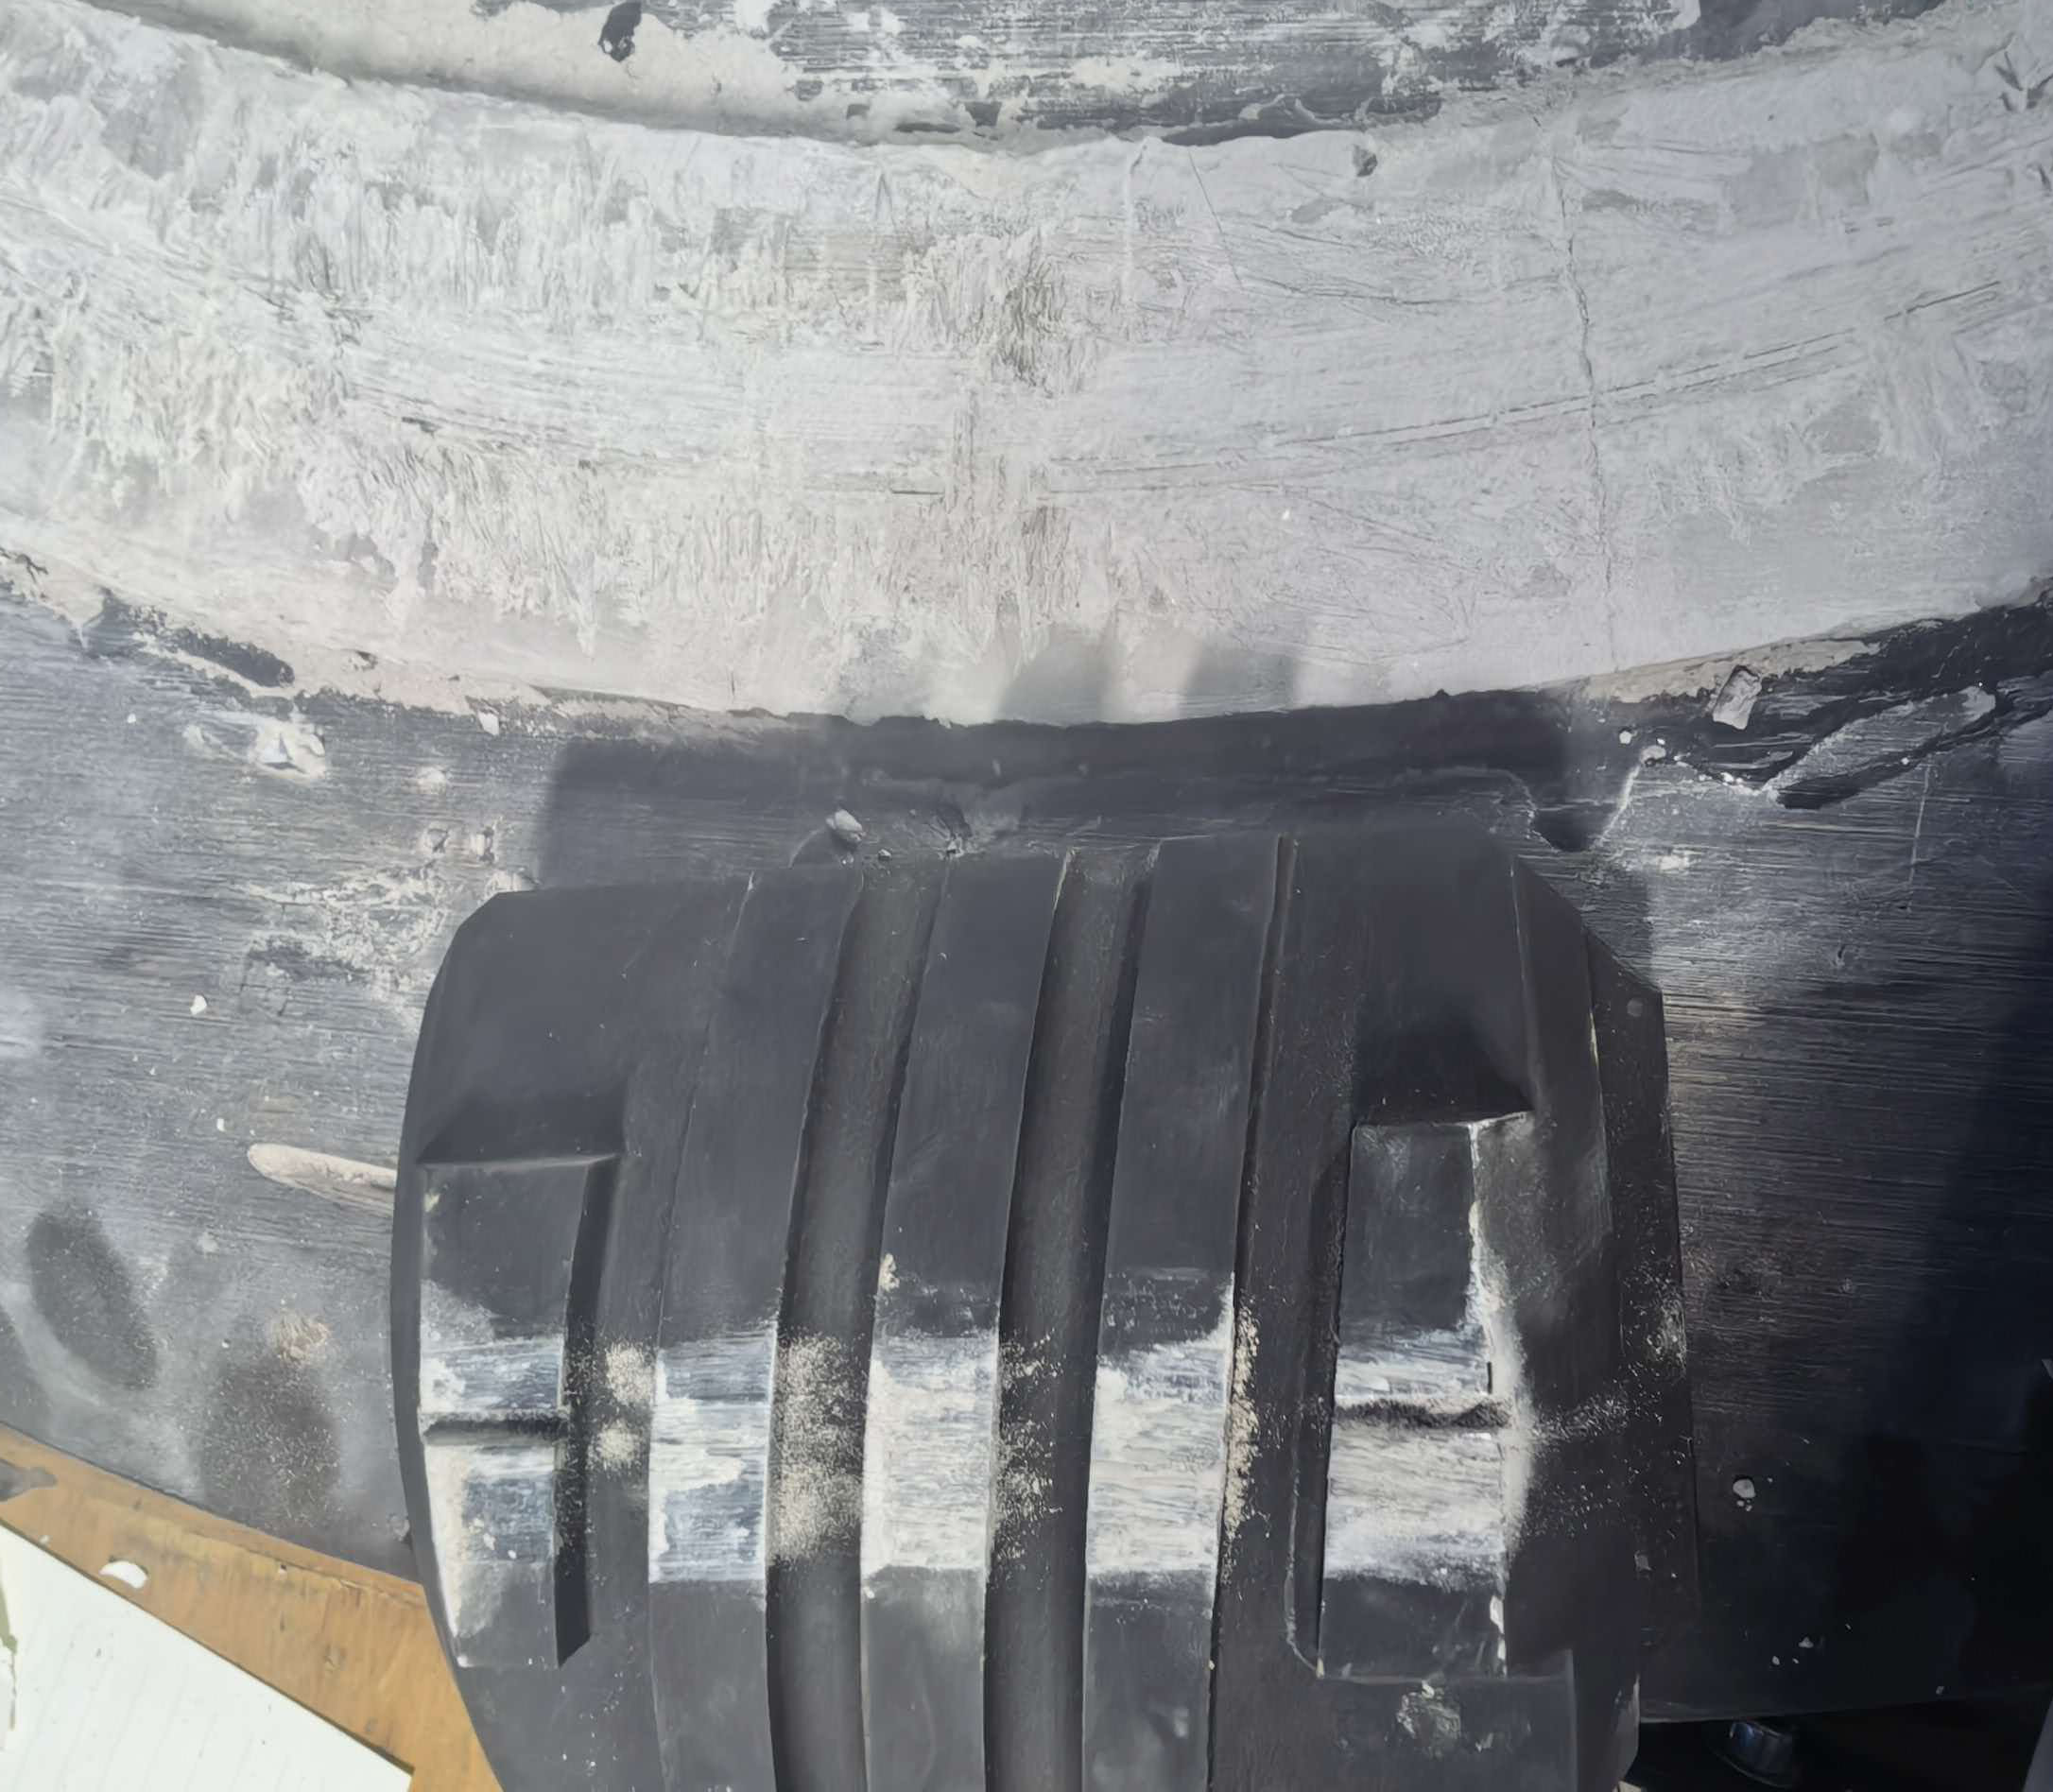
\includegraphics[height=4.0cm]{figure/chapter3/xiechiguaban/1.png}
	\label{fig:helical_scale_1}
	}
	%\hfill
	\subfloat[$\delta_s=10.11\textrm{mm}$]{%
	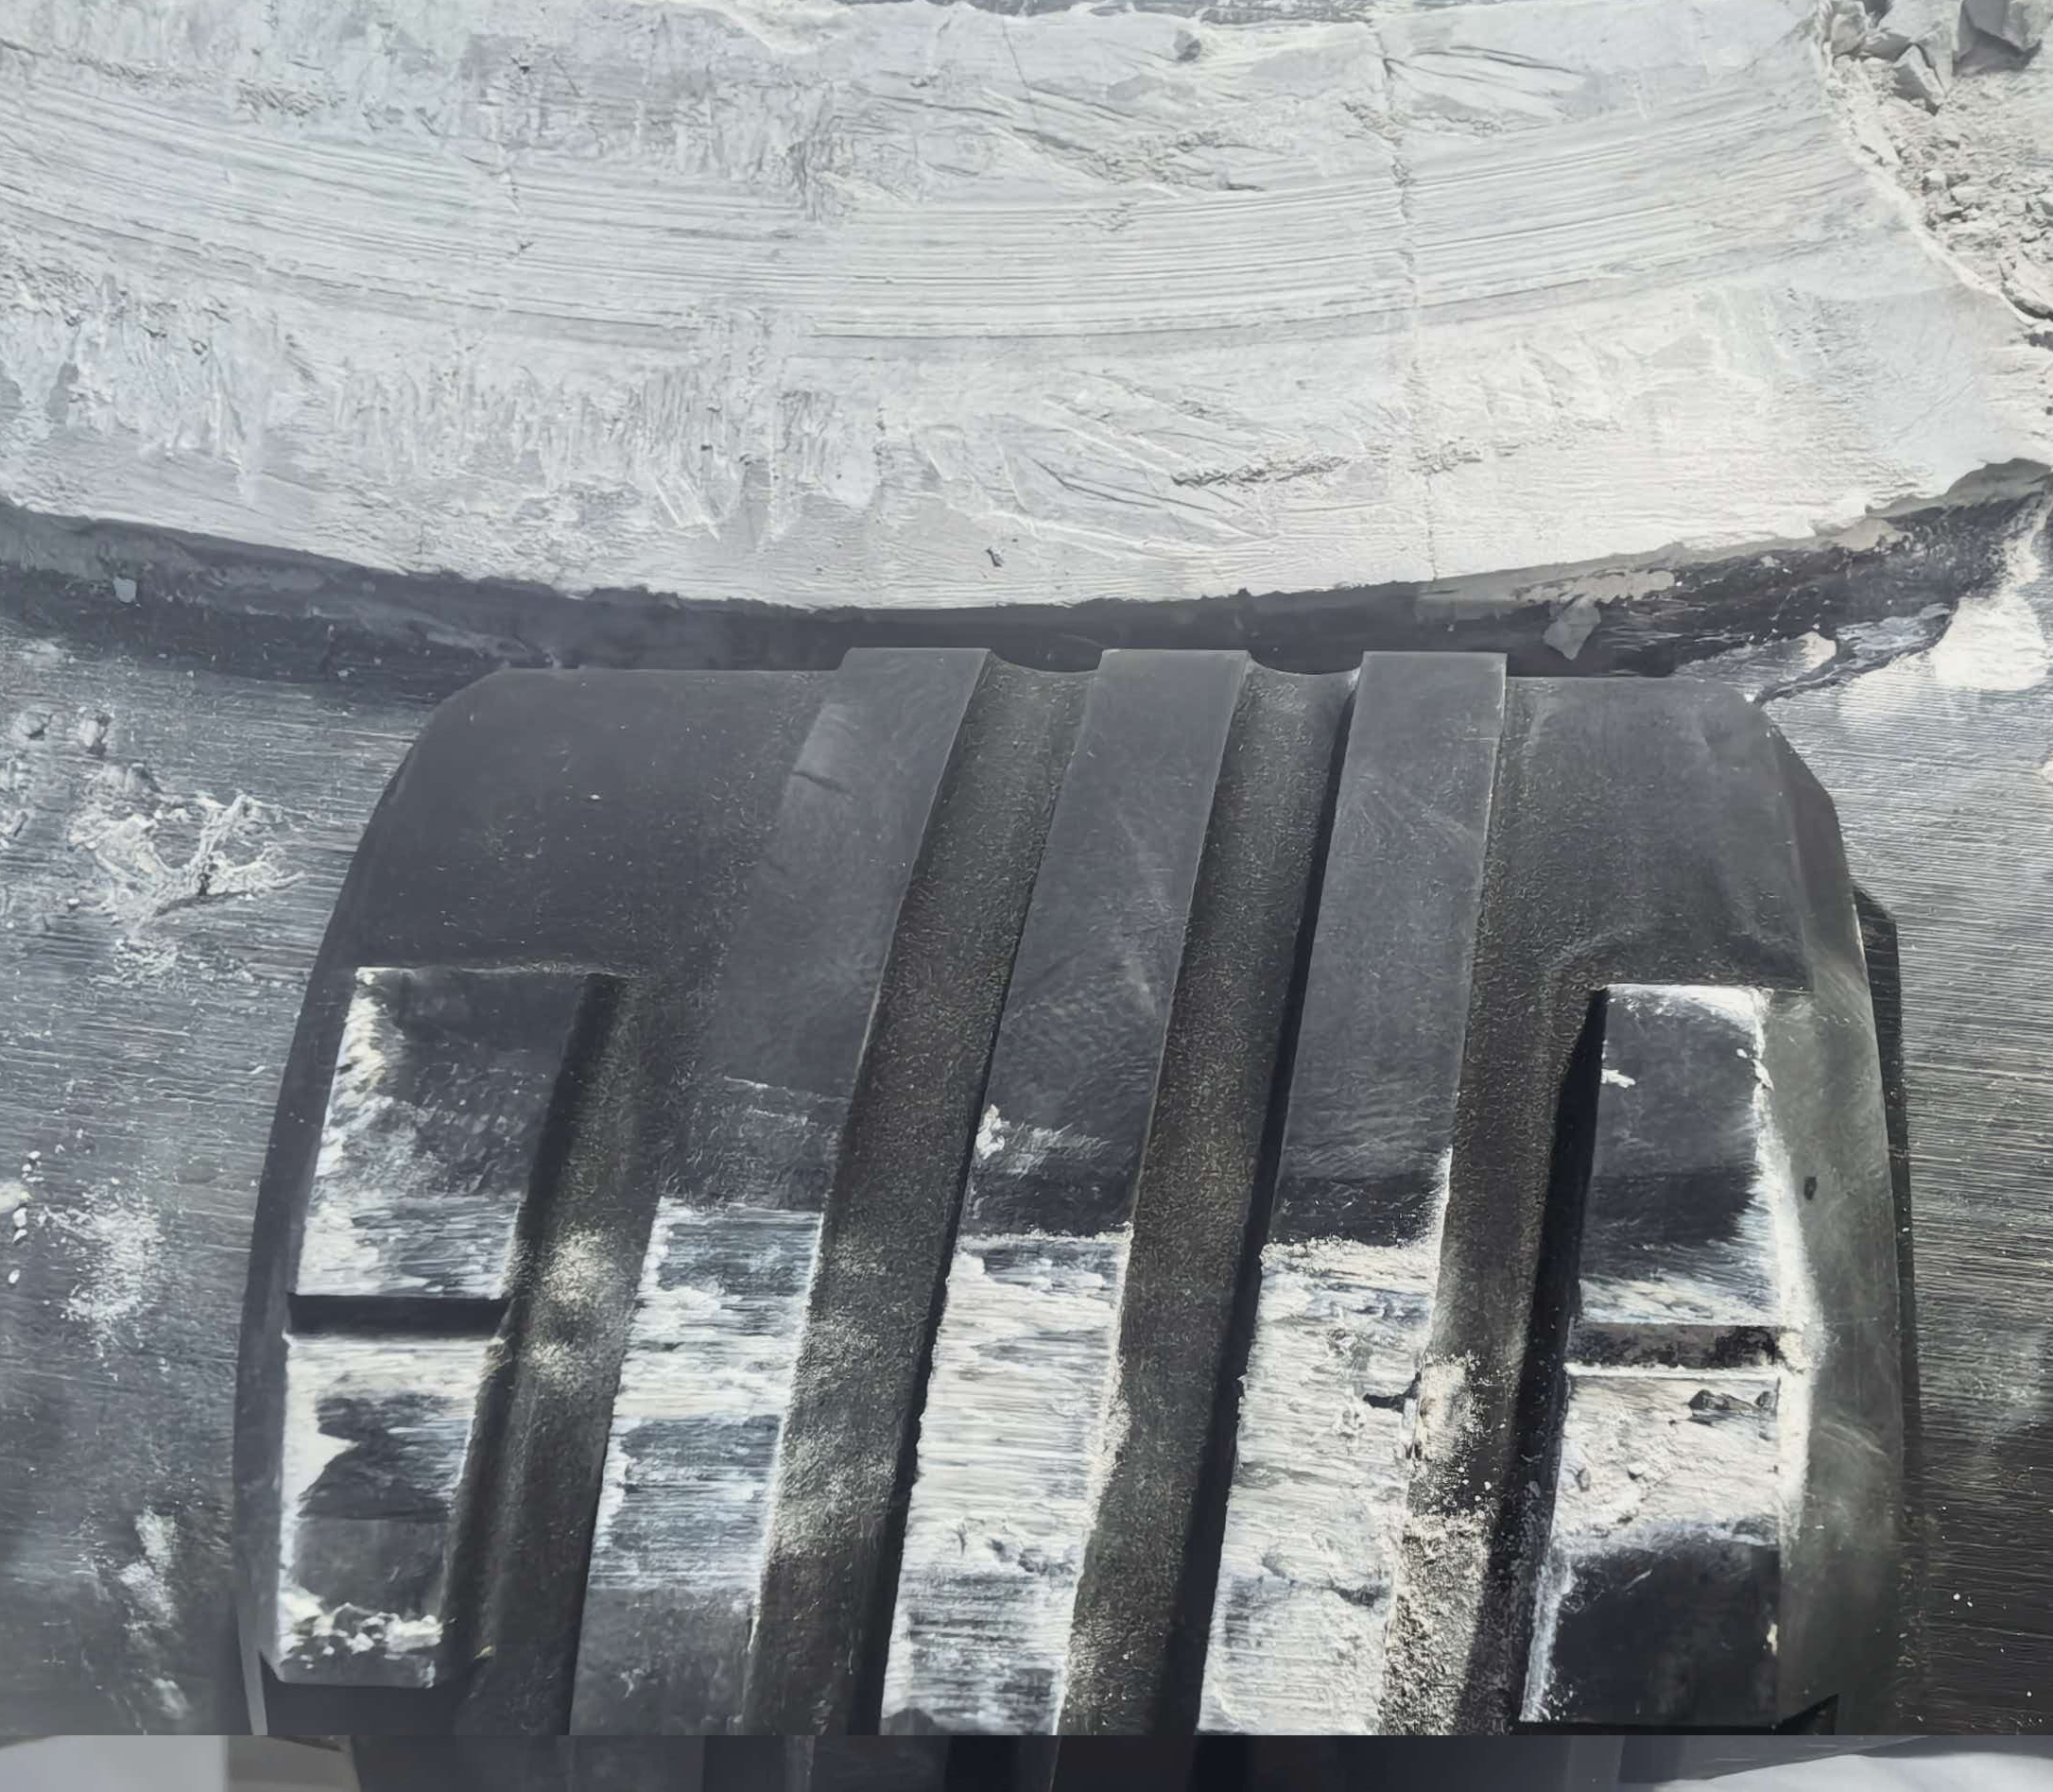
\includegraphics[height=4.0cm]{figure/chapter3/xiechiguaban/2.png}
	\label{fig:helical_scale_4}
	}
	\\[.4em]
	\subfloat[$\delta_s=10.83\textrm{mm}$]{%
	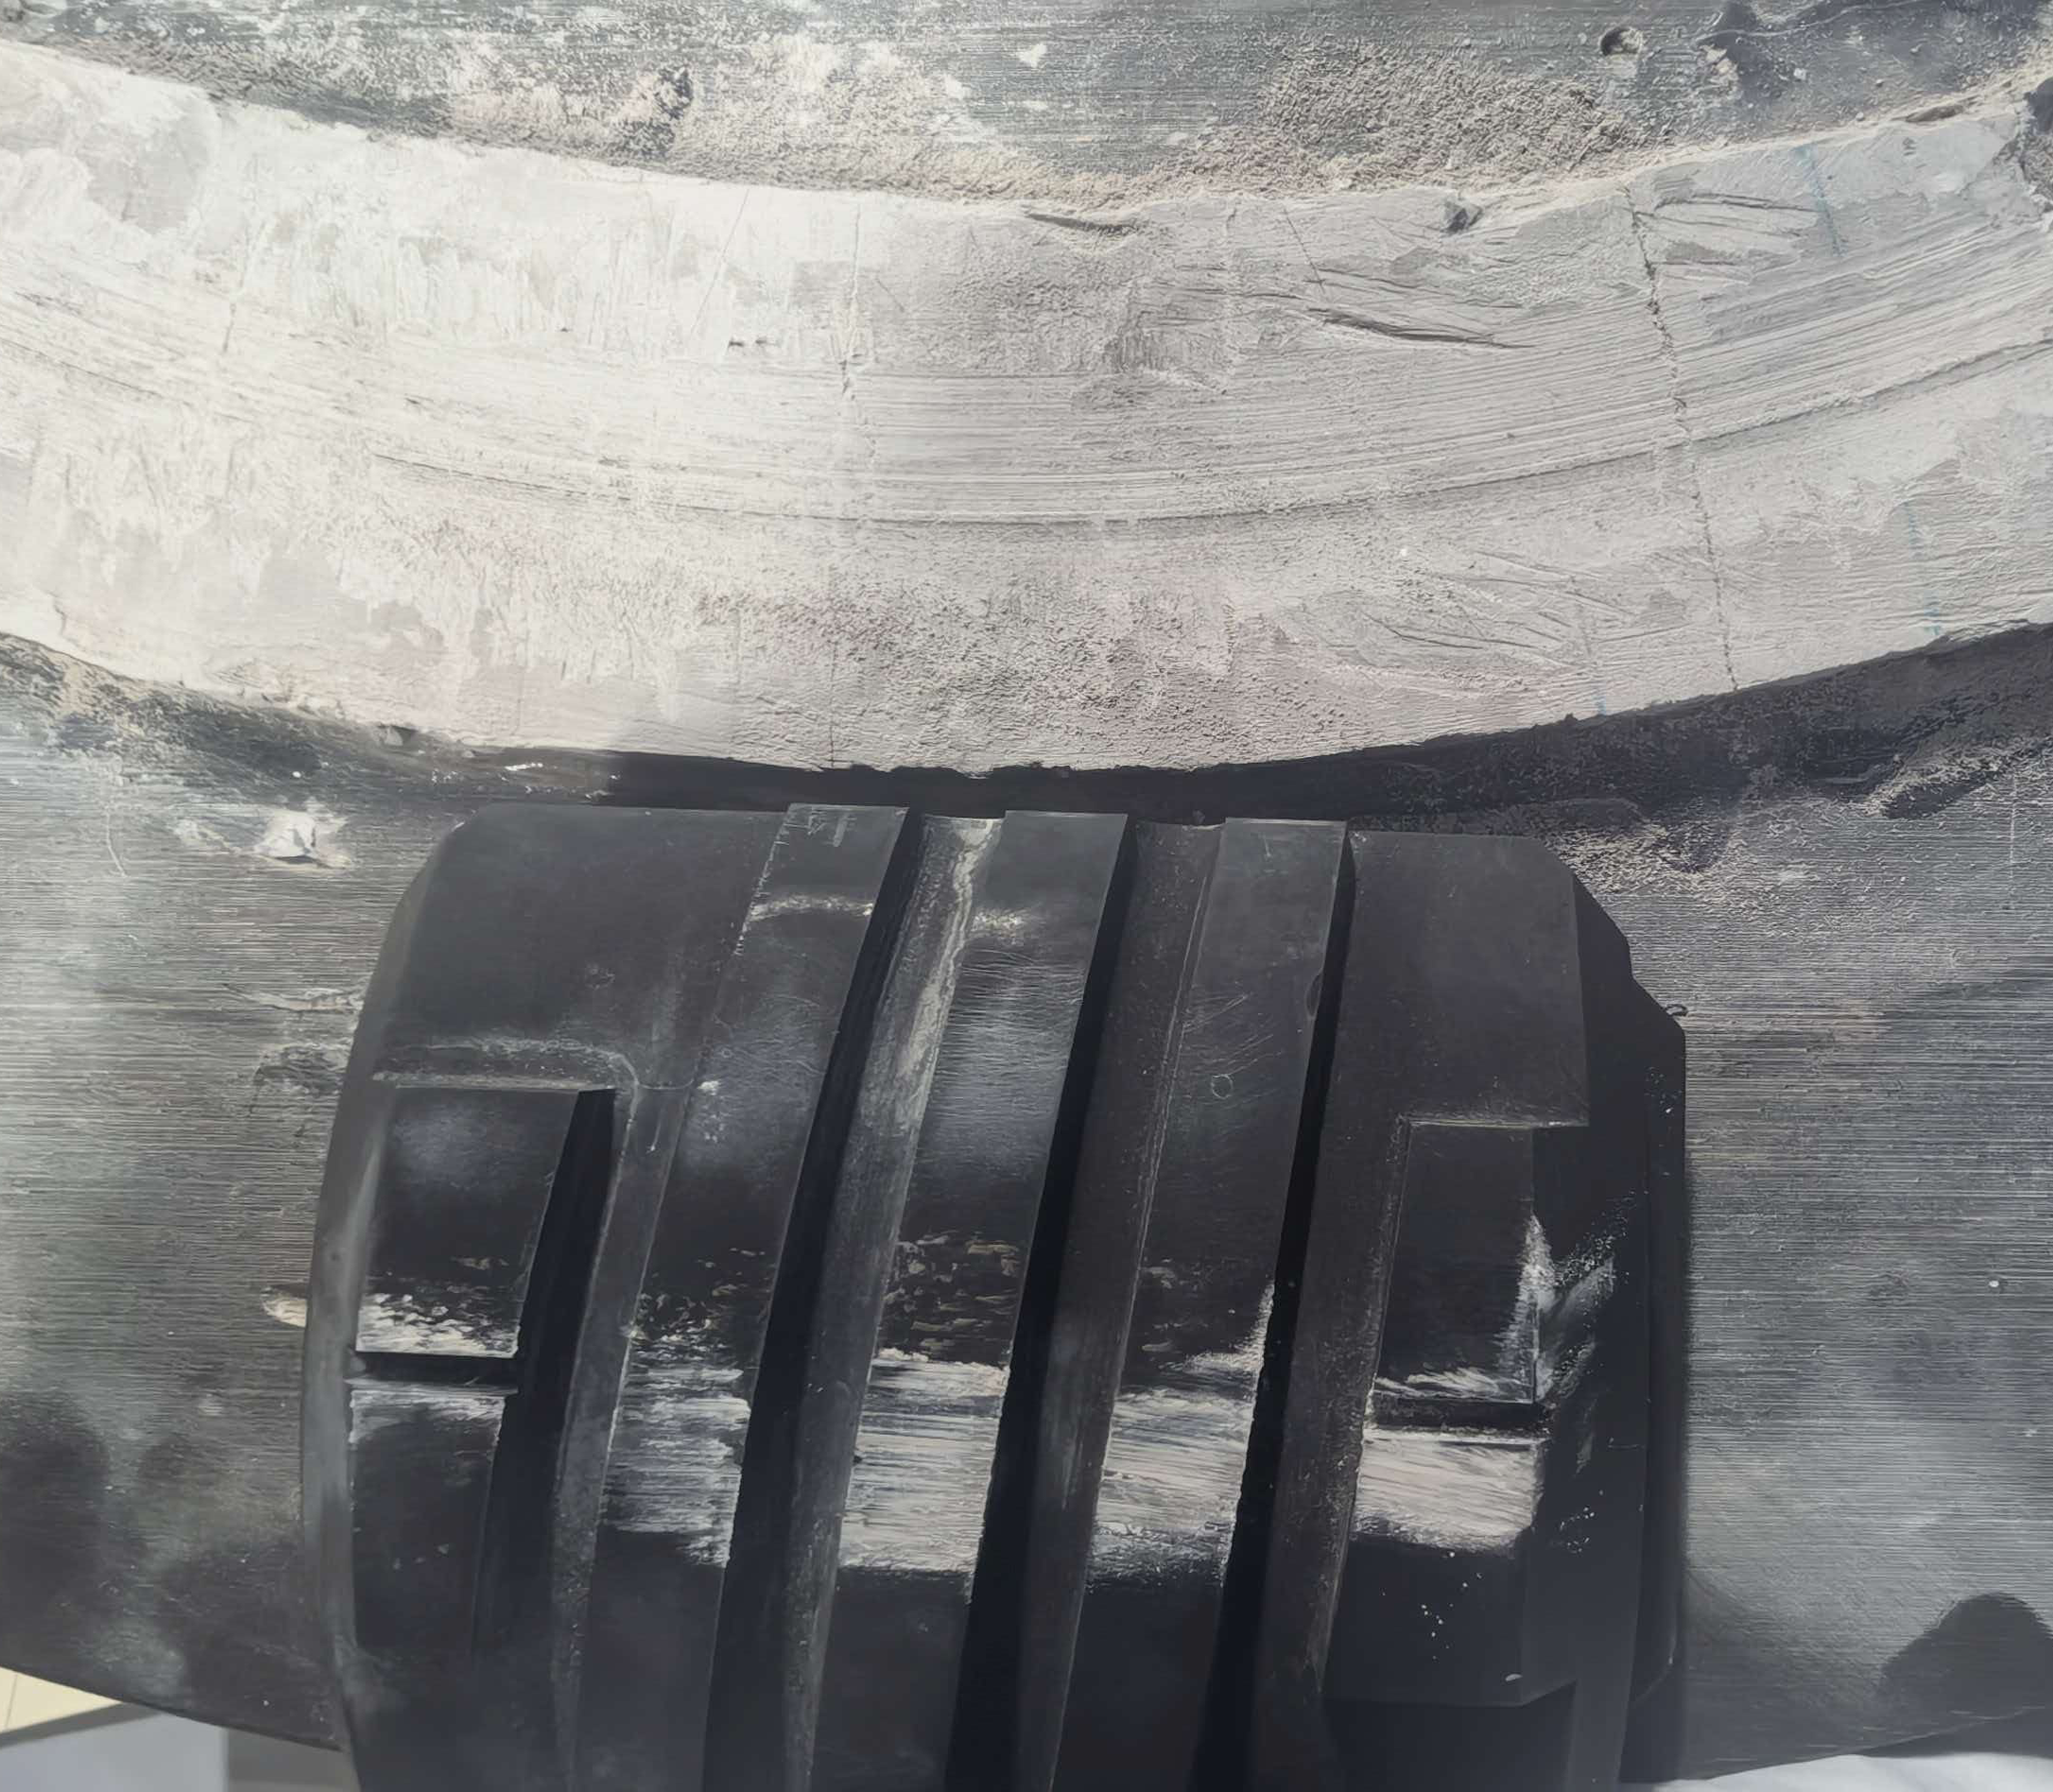
\includegraphics[height=4.0cm]{figure/chapter3/xiechiguaban/3.png}
	\label{fig:helical_scale_3}
	}
	%\hfill
	\subfloat[$\delta_s=11.26\textrm{mm}$]{%
	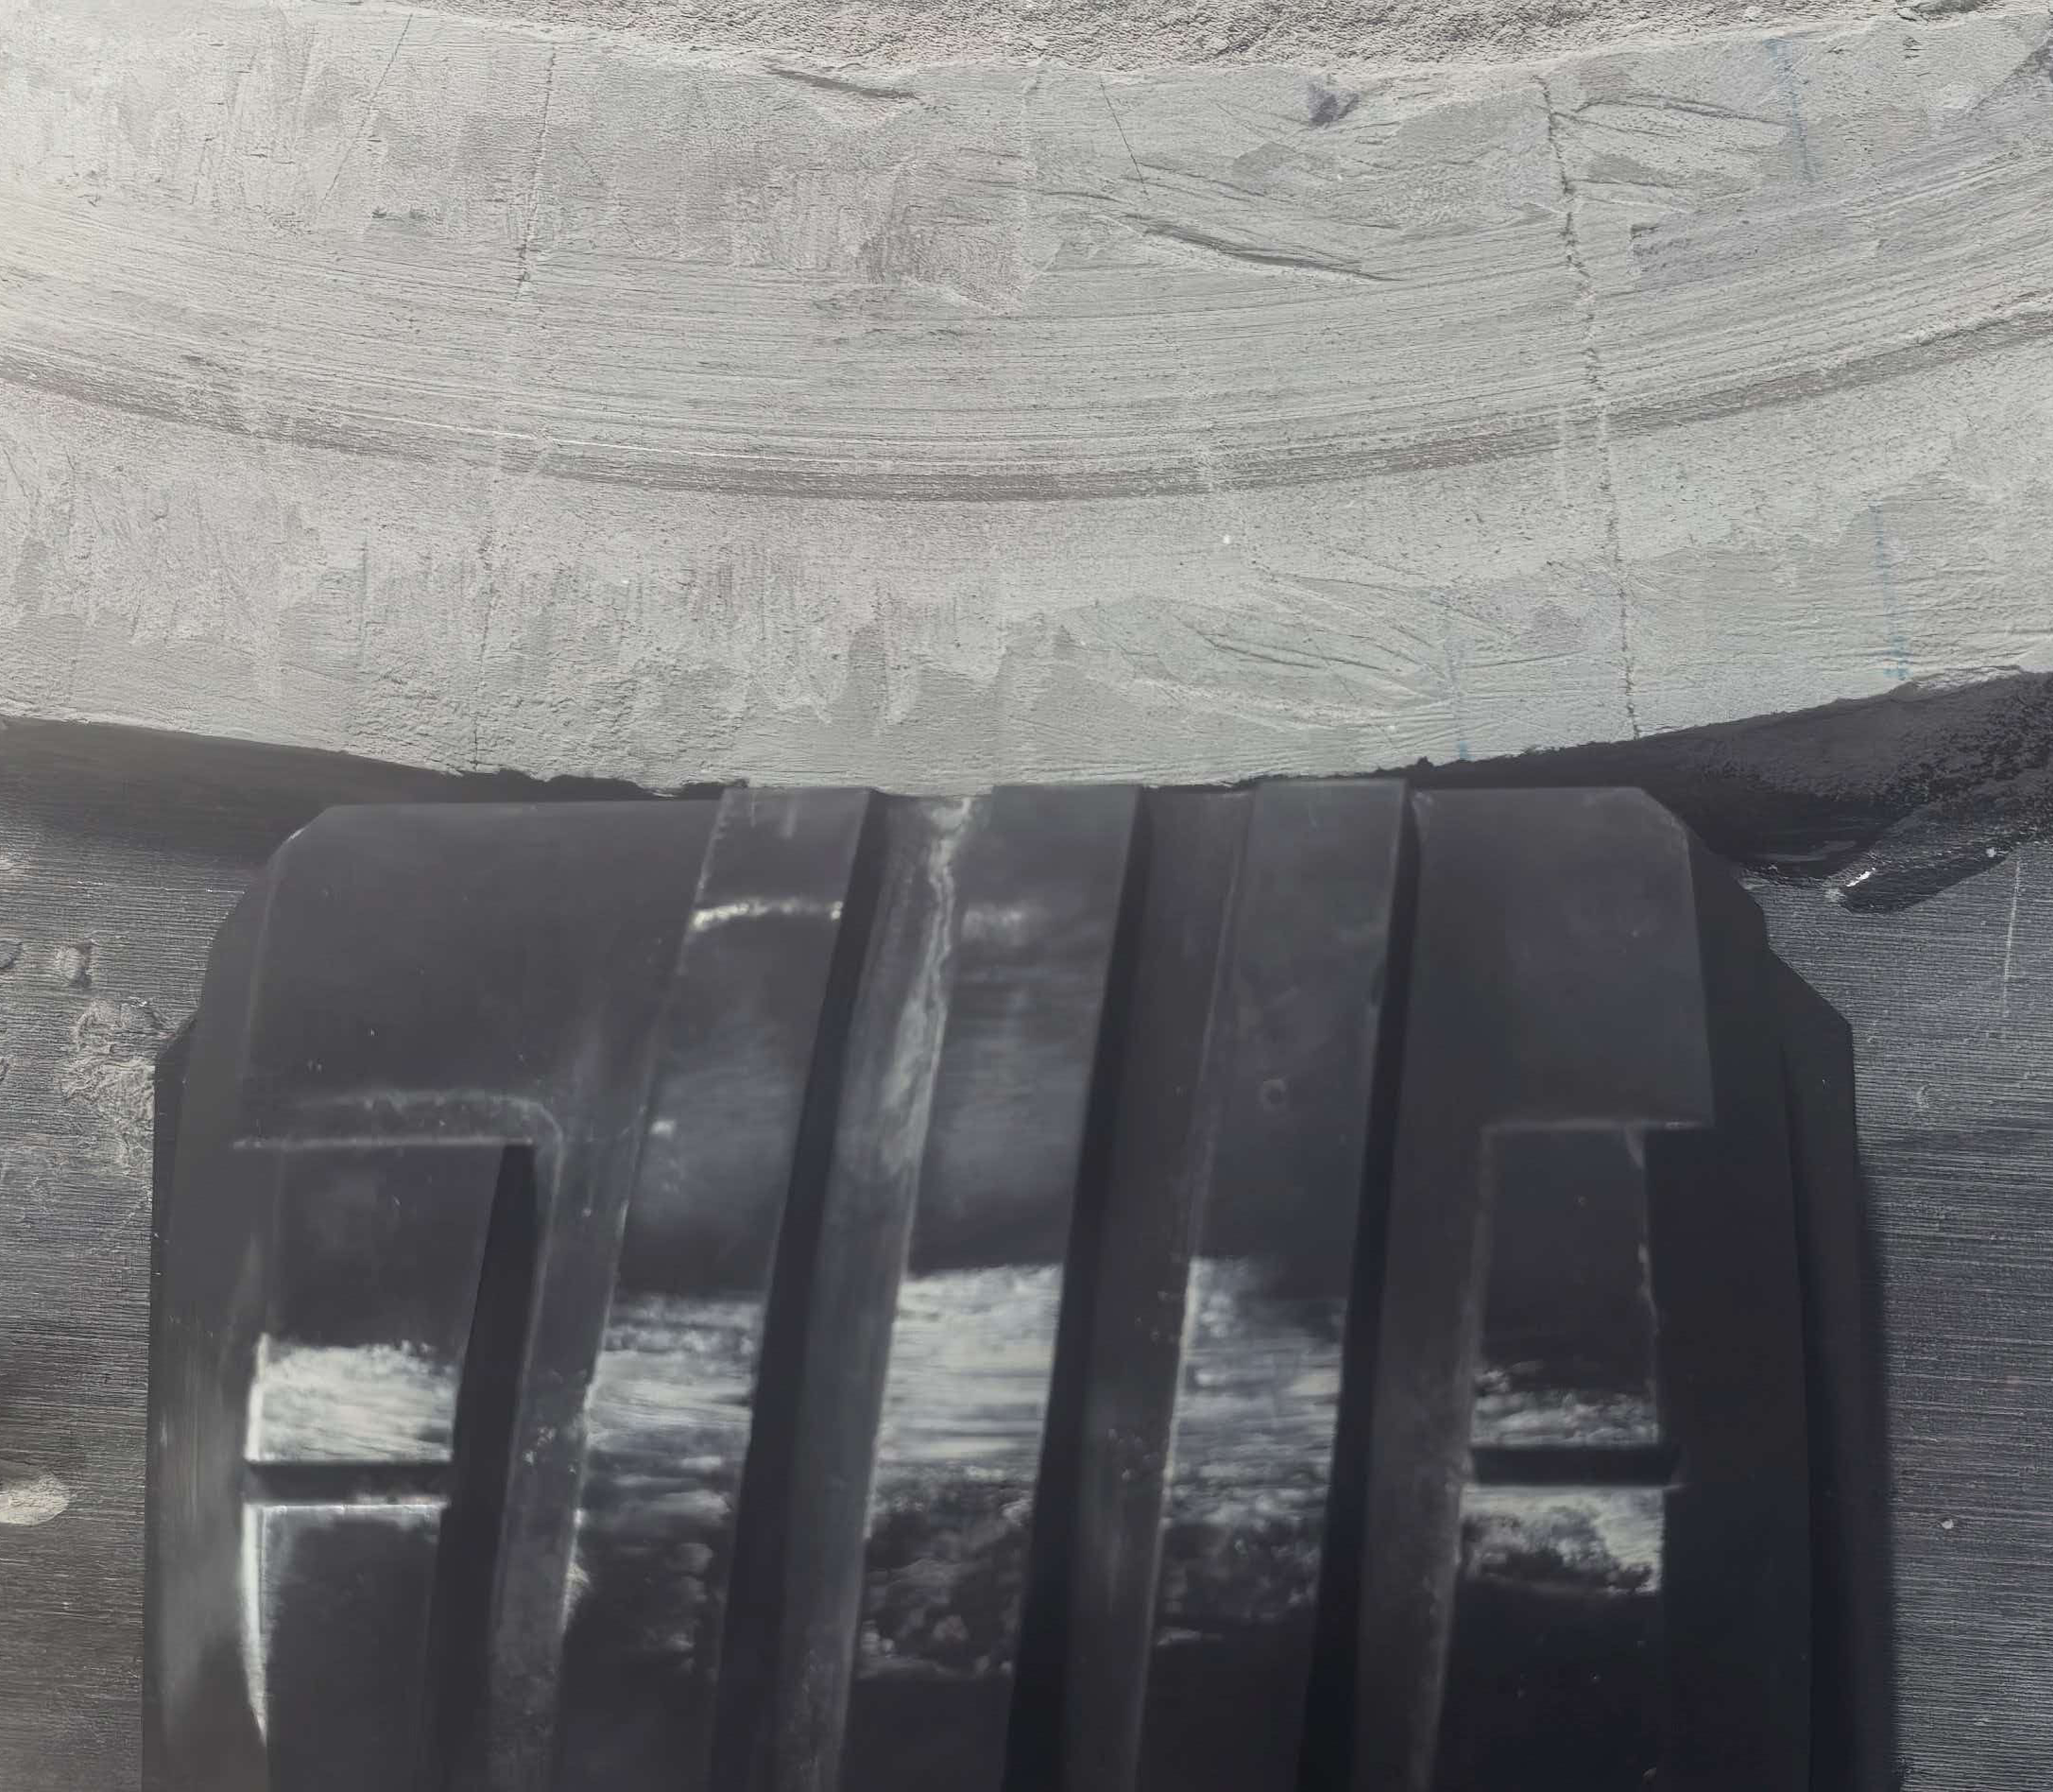
\includegraphics[height=4.0cm]{figure/chapter3/xiechiguaban/4.png}
	\label{fig:helical_scale_5}
	}	
	\caption{垢层经刮削后的表面形貌（不同弹簧压缩量）}
	\label{fig:helical_scale_profile}
\end{figure}

\begin{table}[htbp]
	\centering
	\caption{不同弹簧压缩量下的累积坑深与单次刮削厚度}
	\label{tab:scratch_depth_helical}
	\begin{tabularx}{0.9\textwidth}{CCCCCC}
		\toprule
		工况 & 1 & 2 & 3 & 4 & 5 \\
		\midrule
		弹簧压缩估计值$\delta_s$（mm） & 7.21 & 9.68 & 10.11 & 10.83 & 11.26 \\
		累积坑深$\delta'_c$（mm） & 0.235 & 0.385 & 0.68 & 0.73 & 0.88 \\
		单次刮削厚度$\delta_c$（mm） & 0.235 & 0.15 & 0.295 & 0.05 & 0.15 \\
		\bottomrule
	\end{tabularx}
\end{table}

从单次刮削厚度随弹簧压缩量的响应看（图\ref{fig:helical_scratch_depth_spring_comprassion}、表\ref{tab:scratch_depth_helical}），本次试验共测得5个工况，对应的弹簧压缩估计值$\delta_s$分别约为7.21 mm、9.68 mm、10.11 mm、10.83 mm和11.26 mm，相应的单次刮削厚度约为0.235 mm、0.15 mm、0.295 mm、0.05 mm和0.15 mm。与菱形刮板不同，斜齿形刮板的单次刮削厚度并不随弹簧压缩量的增大而单调增大，而是在$0.05\sim0.295$ mm之间波动：$\delta_s$由7.21 mm增大至9.68 mm时，单次刮削厚度由0.235 mm降至0.15 mm；$\delta_s$继续增大至10.11 mm时回升并达到全试验的最大值0.295 mm，约为9.68 mm工况的2.0倍；$\delta_s$增大至10.83 mm时急剧下降至最小值0.05 mm，仅为最大值的约17\%；$\delta_s$进一步增大至11.26 mm时又回升至0.15 mm，约为最小值的3倍。可见在本试验的$7.21\sim11.26$ mm范围内，斜齿形刮板的单次刮削厚度呈非单调的波动响应，最大值出现在$\delta_s$约为10.11 mm处，最小值出现在$\delta_s$约为10.83 mm处，二者相差约5.9倍。需要说明的是，本试验单次刮削厚度的绝对值较小（$0.05\sim0.295$ mm），与游标卡尺0.02 mm的分辨率处于同一量级，相邻工况之间的差异除受预紧量影响外，还可能叠加测量误差与垢面局部不均匀性的影响，上述波动规律尚需通过重复试验进一步确认。

上述结果表明，在本试验的预紧量范围内，斜齿形刮板的单次刮削厚度受刀齿压入深度、浮动支撑的径向行程余量与齿间排屑条件三者的共同制约，并非随预紧量单调变化。当$\delta_s$小于约9.7 mm时，刀齿的压入深度尚未被充分利用，预紧量的增大主要转化为垢面接触应力的提高与压入深度的增加，单次刮削厚度随之在$9.68\sim10.11$ mm区间内增大并达到峰值；预紧量继续增大后，一方面刀齿逐渐接近浮动支撑的径向行程极限，另一方面垢面被压实变质、齿间产屑量增大（图\ref{fig:helical_scale_profile}），切削所占比重下降、挤压与摩擦所占比重上升，单次刮削厚度在约10.83 mm处降至最低；此后再增大预紧量，垢面形貌与齿间排屑状态随之改变，有效参与切削的齿数有所恢复，单次刮削厚度又回升至0.15 mm。由于本试验中单次刮削厚度的绝对值较小，上述波动中相邻工况之间的差异与测量误差、垢面局部不均匀性处于同一量级，其规律性有待重复试验验证。需要说明的是，本文各工况在同一扇形垢样、同一沟槽上依次进行，弹簧压缩量随工况逐步调整，图中反映的是弹簧压缩量对单次刮削厚度的总体影响趋势。

与图\ref{fig:scratch_depth_spring_comprassion}所示菱形刮板的响应相比，二者的规律存在明显差异。菱形刮板的单次刮削厚度随弹簧压缩量的增大而单调减小，由0.85 mm降至0.08 mm，并在约7.2 mm处出现陡降，超过该临界值后稳定在0.08 mm左右的低水平，说明其有效刮削能力受预紧量上限的严格限制；斜齿形刮板则呈非单调波动（$0.05\sim0.295$ mm），未出现单一的临界陡降，但在$\delta_s$约为10.11 mm处存在明显的峰值、在$\delta_s$约为10.83 mm处存在明显的谷值。从去除量水平看，两种齿形的差异随预紧量区间而不同：在低预紧段（$\delta_s$约为7.2 mm），斜齿形刮板的单次刮削厚度为0.235 mm，约为菱形刮板同水平预紧量（$\delta_s$约为7.09 mm、0.64 mm）的三分之一，说明斜齿以切向分量切入、单次切削的切除体积相对较小；而在较高预紧段（$\delta_s\geq$9.68 mm），斜齿形刮板的单次刮削厚度平均约为0.16 mm，约为菱形刮板同期水平（约0.08 mm）的2倍，说明菱形刮板在超过临界值后已基本丧失有效切削能力，而斜齿形刮板仍能保持相对较高的单次去除量。产生这一差异的原因主要在于刀齿几何：斜齿形刮板的刀齿沿刮削方向倾斜布置，刀齿与垢面自一侧向另一侧逐渐进入切削，避免了直齿全宽同时切入所带来的冲击载荷；同时齿间容屑与过流空间较大，崩碎屑和细屑能够及时排出，齿面不易被完全充填而失效。由此可以认为，刀齿的齿形与排屑条件，是决定刮板在高预紧量下刮削能力是否急剧衰退的重要因素。

面向工程应用，斜齿形刮板的弹簧压缩量应控制在既能保证刀齿充分压入壁面、又能维持齿间排屑通畅的区间内。按本次试验结果，单次刮削厚度的峰值出现在弹簧压缩估计值约为10.11 mm处，取$9.7\sim10.5$ mm附近作为该刮板预紧量的推荐工作区间较为适宜；应避开约10.8 mm附近的低值工况，该预紧量下的单次去除量仅为0.05 mm，继续增大预紧量既不经济，也会因齿间产屑量增大而加剧齿面堵塞。需要指出的是，低预紧量（约7.2 mm）下斜齿形刮板的单次刮削厚度约为菱形刮板的三分之一，因此在垢层较厚、要求较高单次去除量的井段，宜选用菱形刮板或增加刮削次数，而不宜单纯以提高预紧量的方式追求去除量。此外，预紧量上限应由浮动支撑的径向行程与工具结构（保持架、弹簧座等）限定，不宜超过弹簧的允许压缩量，以免弹簧压并、失去浮动缓冲作用；实际应用中还应结合套管的实际内径（同一公称尺寸不同线重时内径不同）匹配刮刀外径与弹簧预紧量，并考虑套管磨损、椭圆度与井斜等因素对实际预紧量的影响。现场作业宜配合循环冲洗及时排出垢屑，防止细屑在容屑槽内板结、堵塞齿面。

综上，本节仍采用转盘式台架评价斜齿形刮板的刮削能力：转盘以低速带动垢样相对固连于机架的刮板旋转，可在低速准静态条件下复现刮板相对垢面的刮削运动，并通过弹簧压缩量与单次刮削厚度的逐点测量，定量比较不同预紧工况下的刮削效果。刮削形貌表明，斜齿形刮板能够以脆性崩碎的方式有效刮除重晶石/钡锶类硬垢，刮痕连续、规则，崩碎屑主要积聚于两侧齿根部平台及容屑槽内，中部容屑槽的排屑状况较好，反映出斜齿布置在排屑方面的结构优势。单次刮削厚度在$0.05\sim0.295$ mm之间非单调波动，峰值（0.295 mm）出现在弹簧压缩估计值约为10.11 mm处、谷值（0.05 mm）出现在约为10.83 mm处，全程未出现菱形刮板在约7.2 mm处那样的临界陡降；在较高预紧量（$\delta_s\geq$9.68 mm）下斜齿形刮板的单次刮削厚度平均约为0.16 mm，约为菱形刮板同期水平的2倍，说明斜齿形刮板在高预紧工况下仍能保持相对稳定的刮削能力。需要说明的是，单次刮削厚度的绝对值较小，与测量工具的分辨率处于同一量级，上述波动规律尚需重复试验确认。工程应用中，建议将弹簧压缩量控制在约$9.7\sim10.5$ mm的推荐区间内、避开约10.8 mm附近的低值工况，按套管实际内径标定刮刀外径与弹簧预紧量，并配合循环冲洗及时排屑，在保证刮削效率的同时避免盲目增大预紧力所带来的齿面堵塞与磨损加剧。

\begin{figure}	
	\centering
	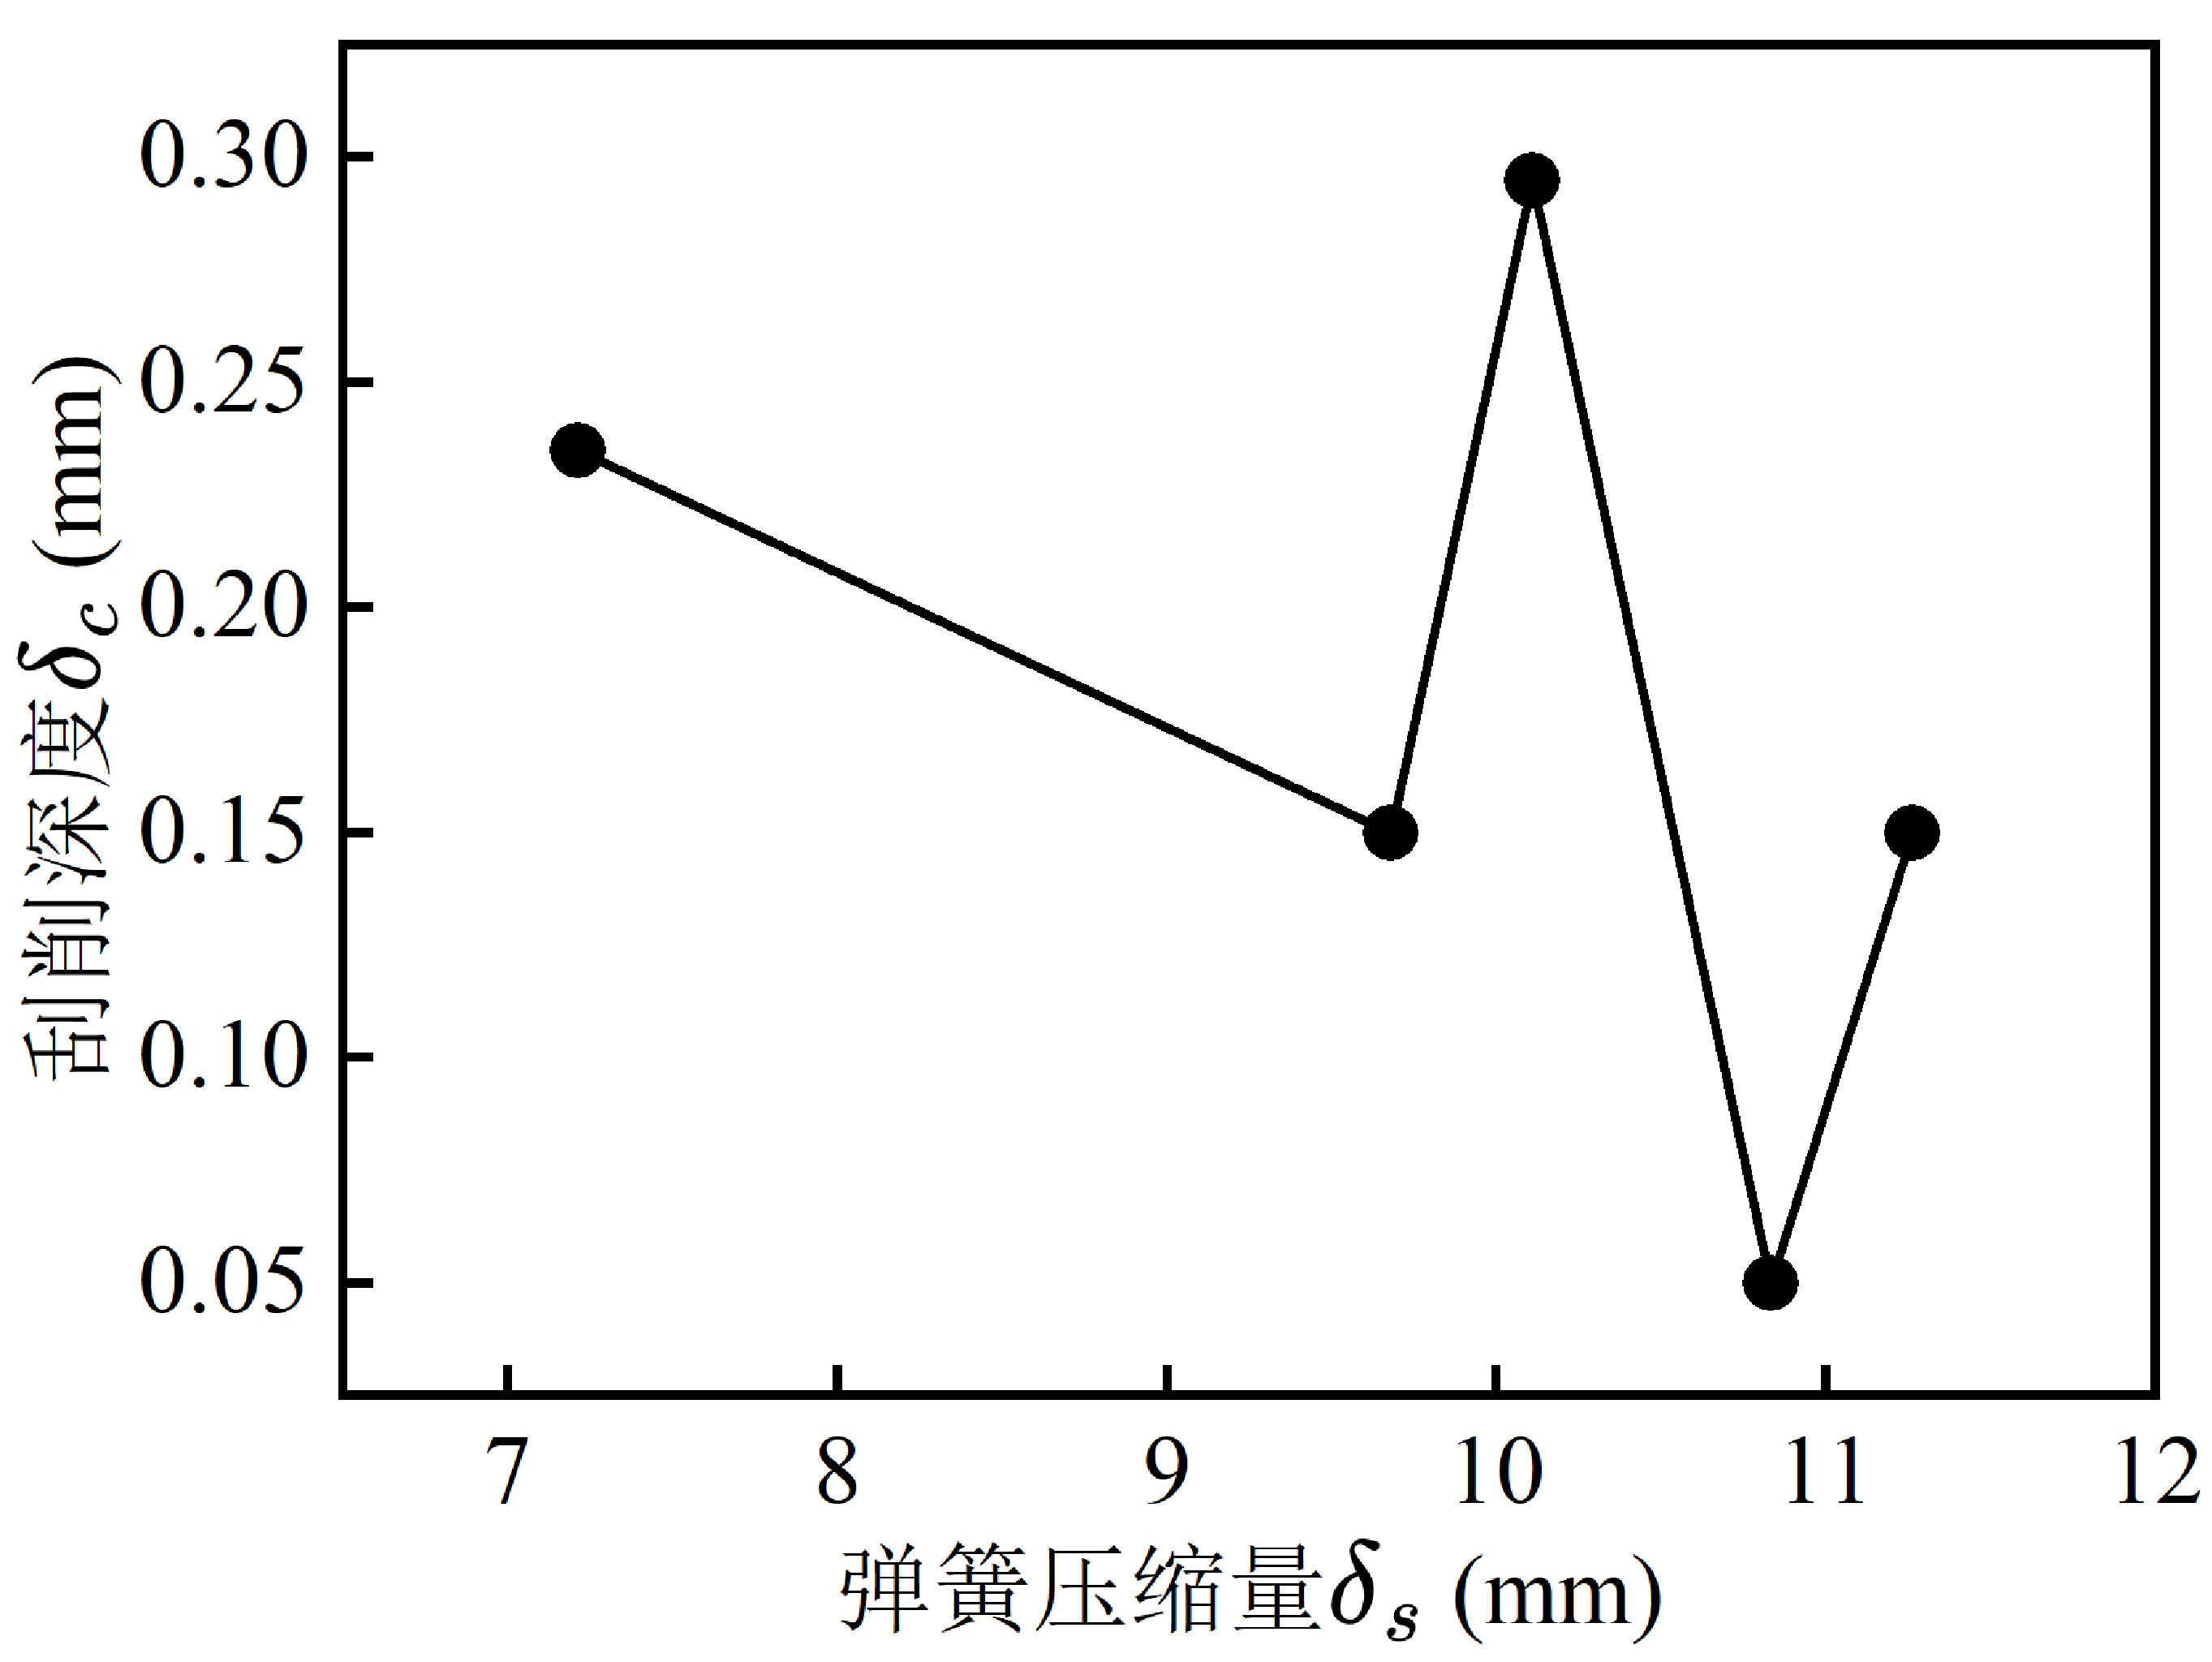
\includegraphics[width=.6 \textwidth]{figure/chapter3/helicle-teetch-scapter-deepth.png}
	\caption{斜齿形刮板刮削厚度与弹簧压缩量之间的关系}
	\label{fig:helical_scratch_depth_spring_comprassion}
\end{figure}
\subsection{毛刷刷洗效果评价}

毛刷模块是四合一工具的后置清扫单元（图\ref{fig:mechanism_swiper_4_in_1}），它安装于刮刀模块之后，利用刷丝与套管壁面的柔性接触清除刮削后残留的细小垢屑与疏松沉积物。刷洗属非切削的接触式清洁，其去除能力与被清除物本身的力学性质密切相关。为明确毛刷刷洗的适用范围，本节在转盘式台架上，以模拟硬垢与模拟蜡垢为对象开展对比刷洗试验，考察同一毛刷块对两类垢层的清洁效果及刷体自身的状态变化。

试验所用垢样与刮板刮削效果评价试验一致，仍以转盘盘面为基体：硬垢试样为以重晶石（硫酸钡）为主的模拟硬垢，蜡垢试样为模拟生产井井筒内的蜡质沉积物。两块垢样在相同条件下先后刷洗，刷洗时毛刷块由刀架夹持并与机架固连，垢样随转盘低速转动，以毛刷刷面相对垢面的滑动实现刷洗，刷洗行程、线速度与刷洗次数均保持一致。刷洗前后分别记录垢面形貌及刷体状态，结果如图\ref{fig:brush_wax_scale}与图\ref{fig:brush_hard_scale}所示。两类垢样各做一次刷洗试验，定量测量沿用刮板试验所用的游标卡尺（分度值0.02 mm），以盖板顶面的测量基面为基准、测至转盘盘面的距离：试验前先在弹簧原长状态下测量测量基面与限位块顶部之间的距离，取4个测点并记为$L_{11}\sim L_{14}$；随后按预定压缩量将弹簧预紧，再次测量同一批测点并记为压缩后的$L_{11}\sim L_{14}$，由二者的差值给出弹簧压缩量$\Delta L_1$与刷块压紧力的标称估算值。同时测量测量基面与垢面之间的距离，取4个测点并记为$L_{21}\sim L_{24}$，以压缩后与刷洗后该测值的均值之差$\Delta L_2$反映刷洗对垢面的作用。其中蜡垢试样的垢层厚度（最高处与最浅处相对高度之差）实测约6.69 mm。毛刷块在两组试验中为同一块，安装方式与刷洗参数均保持一致，两类垢样弹簧压缩量的差别来自弹簧的预紧程度，实测结果汇总于表\ref{tab:brush_test_comparison}。

\begin{figure}[htbp]
	\centering
	\subfloat[刷洗前]{%
	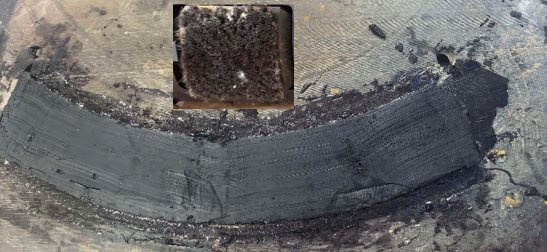
\includegraphics[height=3.6cm]{figure/chapter3/maoshuashiyan/brush-wax-scale-before.jpg}
	}
	\hfill
	\subfloat[刷洗后（含取出的毛刷块）]{%
	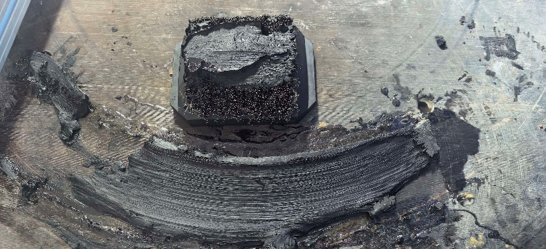
\includegraphics[height=3.6cm]{figure/chapter3/maoshuashiyan/brush-wax-scale-after.jpg}
	}
	\caption{蜡垢刷洗前后的盘面形貌与毛刷块状态}
	\label{fig:brush_wax_scale}
\end{figure}

\begin{figure}[htbp]
	\centering
	\subfloat[刷洗前]{%
	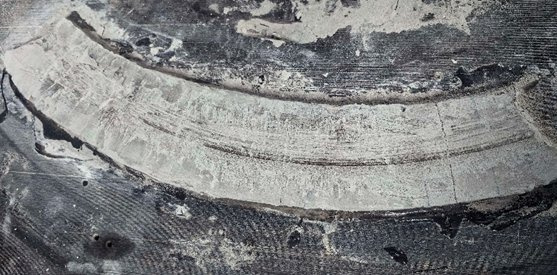
\includegraphics[height=3.5cm]{figure/chapter3/maoshuashiyan/brush-hard-scale-before.jpg}
	}
	\hfill
	\subfloat[刷洗后]{%
	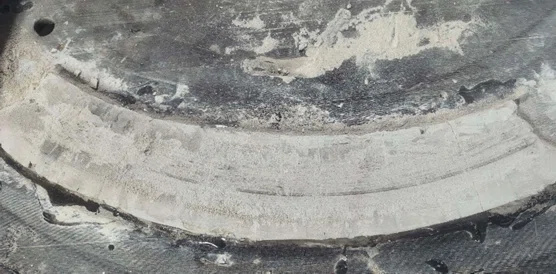
\includegraphics[height=3.5cm]{figure/chapter3/maoshuashiyan/brush-hard-scale-after.jpg}
	}
	\caption{硬垢刷洗前后的垢面形貌}
	\label{fig:brush_hard_scale}
\end{figure}

两次试验的定量结果汇总于表\ref{tab:brush_test_comparison}。硬垢试样在刷洗前将弹簧由22.58 mm压缩至16.45 mm，弹簧压缩量$\Delta L_1$为6.13 mm，按预紧弹簧刚度（22.5 N/mm）估算的刷块压紧力约138 N；压缩后$L_2$测值由原长状态的94.08 mm降至89.51 mm，减小4.57 mm，说明压紧后毛刷端面已随盖板下移并贴紧垢面。在此基础上完成刷洗后再测，$L_2$均值为89.26 mm，仅比压缩后低0.25 mm，即毛刷端面在刷洗过程中几乎没有继续向垢面内推进。蜡垢试样的弹簧压缩量$\Delta L_1$为14.06 mm，刷块压紧力估算值约316 N，约为硬垢试样的两倍以上；但其$L_2$在刷洗后反而由79.13 mm略增至79.92 mm，变化量仅$+0.79$ mm，与毛刷受弹簧压紧的趋势相反，反映的是垢面被刷丝推挤涂抹、局部降低，而非刷丝切入垢层。

\begin{table}[htbp]
	\centering
	\caption{毛刷对模拟硬垢与模拟蜡垢的刷洗对比试验结果}
	\label{tab:brush_test_comparison}
	\begin{tabularx}{1.\textwidth}{CCCCCC}
		\toprule
		\multirow{2}{*}{垢样类型} & 弹簧压缩量 & 刷块压紧力 & \multicolumn{3}{c}{毛刷端面位置测值$L_2$（mm）} \\
		 & $\Delta L_1$（mm） & 估算值（N） & 压缩后 & 刷洗后 & $\Delta L_2$ \\
		\midrule
		模拟硬垢 & 6.13 & 138 & 89.51 & 89.26 & $-0.25$ \\
		模拟蜡垢 & 14.06 & 316 & 79.13 & 79.92 & $+0.79$ \\
		\bottomrule
	\end{tabularx}
\end{table}

表中$L_2$为盖板顶面的测量基面至垢面之间的距离，取4个测点的平均值；$\Delta L_2$为同一试样刷洗后与压缩后$L_2$均值之差，负值表示刷洗后毛刷端面相对垢面进一步下移，正值表示相对升高；刷块压紧力由$\Delta L_1$与预紧弹簧刚度（22.5 N/mm）估算得出。由表\ref{tab:brush_test_comparison}可见，硬垢试样在压紧力约138 N的条件下，刷洗前后$L_2$仅相差0.25 mm，不足弹簧压缩量6.13 mm的5\%，即弹簧的预紧位移绝大部分已在毛刷压紧垢面的阶段消耗完毕，刷洗过程并未使毛刷进一步压入硬垢；这与图\ref{fig:brush_hard_scale}的形貌相互印证——刷洗只在垢面留下连续、细密的弧形擦痕，表层疏松部分被刷去，部分碎屑以粉末状脱离垢面并堆积于垢样两侧，而垢层主体始终保持完整，既未出现大面积剥离，也未出现明显的沟槽。可见毛刷对脆性硬垢几乎没有去除效果，其作用仅限于清除垢面残留的疏松碎屑。蜡垢试样的$L_2$变化方向与硬垢相反：在压紧力约316 N、约为硬垢两倍的条件下，刷洗后$L_2$反而略有升高（$+0.79$ mm），说明垢面在刷丝作用下被推挤、涂抹并局部降低，而毛刷端面并未继续下移。形貌上，刷洗方向上的蜡质留下清晰的塑性流动与涂抹痕迹，垢层被推挤、延展并向两侧堆积，刷洗轨迹上形成宽而浅的沟槽，原有油润光泽被破坏；取出的毛刷块上，刷丝间隙已被刮下的蜡质填满，刷丝相互黏连、黏结成团，形成大面积板结体，毛刷块局部表面被蜡质糊成一片，失去刷丝原有的分散、柔性形态。

上述差异源于两类垢层破坏方式的本质区别。模拟硬垢为脆性材料，毛刷与垢面之间的接触应力不足以使垢层本体破碎，刷丝只能在垢面表面划擦，使表层疏松部分崩落；崩落的粉状碎屑粒径小、黏附性弱，既不能被刷丝有效携带，也不易在刷丝间滞留，故刷洗后垢层本体仍保持完整，去除量有限。蜡垢则不同：常温下呈塑性的蜡质沉积物具有显著的黏温效应，屈服后以塑性流动的方式响应外力。毛刷的接触应力由径向浮动弹簧提供（图\ref{fig:spring}、表\ref{tab:spring_parameters_pitch}），其刷丝直径小、数量多，刷丝施加在蜡垢上的应力虽不足以形成切削，却足以使蜡质屈服，蜡质被反复推挤、涂抹，并黏附于刷丝表面不断转移，由刷丝直接带离垢面；正是这种“黏附—转移”机制，使毛刷对塑性蜡垢具有明显的去除效果，而对脆性硬垢几乎无效。两者差别不在于接触应力的大小，而在于被清除物能否黏附于刷丝并被携带离开垢面。需要说明的是，试验中取出的毛刷块刷丝间填满并黏结成团，是在无循环条件下的现象；在实际井下作业中，循环洗井液不断冲刷刷丝表面，可将黏附于刷丝上的蜡质及时带走，使刷丝免于板结并持续保持柔性。从这个角度看，试验中出现刷体板结的无循环工况，正是井下工况的反面：井下持续流动的洗井液恰能消除试验中观察到的刷丝堵塞。从刷丝与弹片的受力关系看，刷丝本身是弹性体，其压缩变形与径向浮动弹簧构成串联的弹性环节，刷丝与垢面之间实际能达到的接触应力由二者的刚度关系共同决定：弹簧预紧量增大时，外加位移大部分由刷丝的弯曲与压缩变形吸收，转化为刷丝压入垢面深度的部分有限，这为上述定量结果中刷洗效果对预紧量不敏感的现象提供了力学解释。

由此可见，毛刷对硬垢与蜡垢的刷洗效果存在明显差异：对以重晶石/钡锶类矿物为主的脆性硬垢，毛刷几乎无效，刷洗后垢层主体仍然完整，去除量十分有限，其作用仅局限于清除刮削后残留的疏松碎屑；对常温下呈塑性的蜡垢，毛刷则相当有效，蜡质在刷丝作用下被推挤、涂抹并黏附于刷丝表面被带离垢面，去除较为均匀。两类垢样的定量结果还表明，毛刷的去除能力并不取决于弹簧压紧力的大小：硬垢试样在压紧力约138 N的条件下刷洗，$L_2$仅比压缩后低0.25 mm，毛刷几乎没有进一步压入垢面；蜡垢试样的压紧力增至约316 N、约为硬垢的两倍以上，刷洗后$L_2$反而略有升高，反映的是蜡质被推挤涂抹、垢面局部降低，而非刷丝切深增大。两类垢样在压紧力成倍变化的条件下均未出现刚性刮板那种“预紧量越大、切深越大”的比例关系，说明毛刷的有效作用深度主要由毛刷块自身的结构尺寸与刷丝的压缩刚度决定，弹簧预紧量的调节作用有限。

上述定量规律可以从刷丝与垢面的接触状态得到解释。毛刷块通过径向浮动弹簧压紧于垢面，弹簧仅提供压紧力，而真正与垢面接触的是大量细而密的刷丝；刷丝在接触压力下发生弯曲与压缩，其等效刚度与弹簧刚度构成串联，弹簧每增加一定压缩量，刷丝自身即吸收其中相当一部分位移，能够传递到刷丝尖端并转化为有效压入深度的部分十分有限。因此增大弹簧预紧量带来的主要是刷丝弯曲程度的加深与刷块整体压紧力的提高，而不是刷丝尖端压入垢面深度的成比例增加，毛刷的去除能力取决于刷丝能否与垢面保持有效接触并把被清除物带离，而不取决于弹簧施加的压紧力。

由此，弹簧预紧量不应作为调节毛刷去除量的手段。工程上宜按刷丝与套管壁面能够建立稳定接触的要求设定预紧量，把预紧量控制在足以保证有效接触并补偿刷丝磨损的适度范围内，而将去除能力的调节交给刷丝参数（直径、伸出长度、布置形式与数量）和刷洗次数、行程等工艺参数；对塑性蜡质垢层，则须先由刮板或刮刀切槽破坏垢层连续性，再以毛刷清除被刮松的碎屑，单纯依靠毛刷并盲目增大预紧力无助于提高清洁效果。

面向工程应用，对以塑性蜡质沉积物为主的井段，宜采用“刮削＋刷洗”的协同工艺：先由刮板或刮刀在蜡垢层中切出沟槽、破坏其连续性，再由毛刷清扫被刮松的蜡质碎屑，避免毛刷直接与完整蜡垢大面积接触；必要时可辅以热洗或化学溶剂降低蜡垢黏度与塑性，使其由塑性向脆性转变后再行刷洗。在毛刷结构上，可通过增大刷丝直径与刷丝间距、采用束状或波浪形布置等措施延缓蜡质在刷丝间的滞留与板结；在布置上，宜保证毛刷位于刮削元件之后并适当增大刷丝伸出长度与径向压缩量，以提高有效接触应力，同时便于在生产井作业中通过循环洗井将黏附在刷丝上的蜡质及时带走。


\subsection{操作方式}
\subsubsection{使用方法}
根据井眼尺寸选择合适的套管清洁工具，根据井眼情况选择各模块的数量及排列组合方式。
四合一工具用钻柱送入井底进行清洁作业。
\subsubsection{操作方法}
该工具可以与强磁吸附工具一同使用（推荐），也可以单独使用。
将四合一工具下到井底离通井位置$3\sim 5\mathrm{m}$处，开泵循环。将四合一工具在该位置上下活动。保持循环的情况下，平稳的上提钻柱。
起钻时要求平稳、低速、严禁剧烈震动与撞击。

\subsection{维护与保养}
\subsubsection{保养}
下井使用过的四合一工具必须进行保养及维修，在钻台现场进行保养是在井场钻台上起出井后，四合一工具外表面和水眼内的泥浆。

\subsubsection{管子站维修}
建议：在井下正常运转400小时后的四合一工具应送管子站进行大修，必须更换所有密封件和易损件，工具大修三次后报废。外筒零件磨损量（或偏磨量）大于产品外径尺寸1\%时，该套管清洁工具报废。修前应准备好下列设备、工具、附件：适用于该工具尺寸的链钳、管钳、手钳等相应工具；起重吊车、固定钳、稳定座、拆装架，试验架等设备；清洗用的煤油等；各种所需的润滑脂、润滑油等。

\subsection{测试与检查}

刮削器所用金属材料如需作力学性能试验，应按GB/T228的有关规定进行。刮板寿命按照SY/T 5110-2000进行刮刀寿命测试，刮削器的刮削寿命试验应在模拟试验台上进行。选用500号硅酸盐水泥，在对应的试验套管内壁上候凝24h。将试验套管固定在试验台底座上，将刮削器接到试验台的钻杆上，加压压力$0.8\sim10\mathrm{kN}$，用$36\mathrm{r/min}$的速度进行模拟刮削，每次刮削1h，刮削3次。然后拆检测量刀体的磨损量，用渐进法验证其寿命。

四合一工具拆卸后应尽快进行检查，更换不满足使用条件的配件，不能采用非原厂配件。清洗前的检查，肉眼检查外部零件的损坏并记录异常磨损或作记号。如果发现明显损伤，需要对配件进行特别处理。清洗，用水浸泡零件以除掉干的结块和泥浆。用蒸汽和强力生物清洁剂去掉油和黄油。配件干燥、冷却后进行检查。

每次套管清洁工具被拆开时，用下述步骤检查所有配件。按API标准检查所有的接头螺纹，检查步骤要符合API标准。检查所有的配合面和端面是否清洗和有无磨损，需要时，修理和更换配件。检查所有外部配件是否磨损，当外径磨损超过尺寸的1\%以上时， 更换配件。配件有超过最小磨损量的凹槽或缺口不能继续使用，在一个小区域有许多凹槽 或缺口也不能再使用，要求更换配件。探伤检查，每次维修时，对所有受力件进行超声波或磁粉探伤检查，如果发现裂缝和伤痕指示，而且不能被修复的，则更换配件。用新、修理过的或继续使用的配件进行装配。所有配件须保证整洁。

